\documentclass[aspectratio=169,10pt]{beamer}

\usepackage[spanish]{babel}
\usepackage[utf8]{inputenc}
\usepackage{graphicx}
\usepackage{booktabs}
\usepackage{array}
\usepackage{ragged2e}
\usepackage{tabularx}
\usepackage{tabulary}
\usepackage{longtable}
\usepackage{threeparttablex}
\usepackage{multirow}
\usepackage{multicol}
\usepackage{rotating}
\usepackage{colortbl}
\usepackage{hhline}
\usepackage{adjustbox}
\usepackage{float}
\usepackage{caption}
\usepackage{subcaption}
\usepackage{microtype}
\usepackage{siunitx}
\usepackage{amsmath}
\usepackage{amssymb}
\usepackage{mathtools}
\usepackage{nccmath}
\usepackage{cancel}
\usepackage{gensymb}
\usepackage{wasysym}
\usepackage{marvosym}
\usepackage{calc}
\usepackage{tcolorbox}
\usepackage{newfloat}
\usepackage{enumerate}
\usepackage{enumitem}
\usepackage{etoolbox}
\usepackage{fancyhdr}
\usepackage{comment}
\usepackage{hyperref}
\usepackage{tikz}
\usepackage{pgfplots}
\usepackage{pgfplotstable}
\usepackage{pgf-pie}
\usetikzlibrary{arrows.meta,mindmap,patterns,positioning,shapes.geometric}
\usepgfplotslibrary{dateplot}
\pgfplotsset{compat=1.18}
\sisetup{output-decimal-marker={.}}

\newcolumntype{P}[1]{>{\RaggedRight\arraybackslash}p{#1}}

\usetheme{Singapore}
\usecolortheme{orchid}
\setbeamertemplate{navigation symbols}{}
\setbeamertemplate{headline}{}
\setbeamertemplate{footline}[page number]
\setbeameroption{hide notes}

\title[Finanzas Públicas Colombianas]{Finanzas Públicas Colombianas}
\subtitle{Curso integrado y panorama fiscal}
\author{Oliver Pardo, Andrés Garzón y Gabriel Millán}
\institute{Pontificia Universidad Javeriana}
\date{2026}

\AtBeginSection[]{
  \begin{frame}{Contenido}
    \tableofcontents[currentsection,sectionstyle=show/shaded]
  \end{frame}
}

\begin{document}

\begin{frame}
  \titlepage
\end{frame}

\begin{frame}{Contenido}
  \tableofcontents
\end{frame}

\section{Presentación del curso}
\begin{frame}
  \frametitle{Datos de Contacto}
  \begin{columns}[T,onlytextwidth]
    \begin{column}{0.48\textwidth}
      \begin{block}{Oliver Pardo}
        \textit{Profesor de la clase magistral}\\[0.15cm]
        PhD en Econom\'ia, LSE\\
        Profesor Asociado, FCEA--PUJ\\[0.2cm]
        pardoo@javeriana.edu.co
      \end{block}
    \end{column}
    \begin{column}{0.48\textwidth}
      \begin{block}{Andr\'es Garz\'on}
        \textit{Profesor del taller aplicado}\\[0.15cm]
        An\'alisis de informaci\'on y datos de finanzas p\'ublicas\\[0.2cm]
        garzonandresf@javeriana.edu.co
      \end{block}
    \end{column}
  \end{columns}
  \note{[Sources] ProgramaFPC, Google Doc suministrado por el usuario, consultado el 29 de julio de 2026.}
\end{frame}


\begin{frame}
  \frametitle{Introducci\'on}
  El curso estudia c\'omo funciona y se financia el sector p\'ublico colombiano, c\'omo se asignan y ejecutan los recursos y qu\'e implicaciones tienen estas decisiones sobre:
  \begin{itemize}
    \item el desempe\~no econ\'omico y la estabilidad macroecon\'omica;
    \item la equidad y el desarrollo social;
    \item la sostenibilidad fiscal y la coordinaci\'on intergubernamental.
  \end{itemize}
  Combina teor\'ia econ\'omica, an\'alisis institucional, datos y discusi\'on de pol\'iticas p\'ublicas.
  \note{[Sources] ProgramaFPC, Google Doc suministrado por el usuario, consultado el 29 de julio de 2026.}
\end{frame}

\begin{frame}
  \frametitle{Objetivos del Curso}
  \begin{itemize}
    \item Comprender la estructura institucional y fiscal del sector p\'ublico.
    \item Analizar ingresos y gastos nacionales y territoriales.
    \item Evaluar la sostenibilidad fiscal y sus efectos macroecon\'omicos y sociales.
    \item Interpretar el MFMP, el PGN y los informes del FMI.
    \item Formular argumentos y propuestas de pol\'itica sustentados en evidencia.
    \item Manejar y visualizar datos fiscales con herramientas digitales.
  \end{itemize}
  \note{[Sources] ProgramaFPC, Google Doc suministrado por el usuario, consultado el 29 de julio de 2026.}
\end{frame}

\begin{frame}
  \frametitle{Metodolog\'ia y Evaluaci\'on}
  \begin{block}{Sesi\'on semanal: 4 horas}
    \textbf{3 horas:} clase magistral, quizzes y presentaciones, a cargo de Oliver Pardo.\\
    \textbf{1 hora:} taller de an\'alisis de informaci\'on fiscal, a cargo de Andr\'es Garz\'on.
  \end{block}
  \begin{alertblock}{Evaluaci\'on}
    \begin{itemize}
      \item \textbf{Quizzes: 33,33\%.} Lecturas, clase magistral y presentaciones.
      \item \textbf{Presentaci\'on en grupo: 33,33\%.} Equipos de 2--3 estudiantes; hasta dos horas, incluida la discusi\'on.
      \item \textbf{Taller aplicado: 33,33\%.}
    \end{itemize}
  \end{alertblock}
  \note{[Sources] ProgramaFPC, Google Doc suministrado por el usuario, consultado el 29 de julio de 2026.}
\end{frame}


\begin{frame}
  \frametitle{El curso avanza de la arquitectura fiscal a su aplicaci\'on}
  \small
  \begin{itemize}
    \item \textbf{M0:} Presentaci\'on del curso --- 1 sesi\'on
    \item \textbf{M1:} Conceptualizaci\'on del sector p\'ublico --- 1 sesi\'on
    \item \textbf{M2:} Gobierno Nacional Central --- 4 sesiones
    \item \textbf{M3:} Regla fiscal y ciclo presupuestal --- 1 sesi\'on
    \item \textbf{M4:} Seguridad social en pensiones --- 2 sesiones
    \item \textbf{M5:} Seguridad social en salud --- 1 sesi\'on
    \item \textbf{M6:} Finanzas p\'ublicas territoriales --- 1 sesi\'on
    \item \textbf{M7:} Colombia en el contexto internacional --- 1 sesi\'on
    \item \textbf{M8:} Presentaciones en grupo --- 6 sesiones
  \end{itemize}
  \note{[Sources] ProgramaFPC, Google Doc suministrado por el usuario, consultado el 29 de julio de 2026.}
\end{frame}

\begin{frame}
  \frametitle{Componente Aplicado: Manejo de Datos}
  \begin{itemize}
    \item Base de datos del Gobierno Nacional Central.
    \item PEPE: Presupuesto en Perspectiva Econ\'omica.
    \item GEIH para el an\'alisis de pensiones y protecci\'on social.
    \item SICODIS para distribuciones de recursos territoriales.
    \item Terridata y FUT para finanzas departamentales y municipales.
    \item Visualizaci\'on e interpretaci\'on de indicadores fiscales.
  \end{itemize}
  \note{[Sources] ProgramaFPC, Google Doc suministrado por el usuario, consultado el 29 de julio de 2026.}
\end{frame}

\begin{frame}{M1--M2: del mapa institucional a las cuentas del GNC}
\scriptsize
\begin{columns}[T,onlytextwidth]
  \begin{column}{0.38\textwidth}
    \begin{block}{M1. Sector p\'ublico colombiano}
      \textbf{Obligatorias}
      \begin{itemize}
        \item C\'ardenas (2020), \textit{Introducci\'on a la Econom\'ia Colombiana}, cap. 6.
        \item Lora y Prada (2023), \textit{T\'ecnicas de medici\'on econ\'omica}, cap. 17.
      \end{itemize}
      \textbf{Sugerida:} FMI (2014), \textit{Manual de Estad\'isticas de Finanzas P\'ublicas}.
    \end{block}
  \end{column}
  \begin{column}{0.35\textwidth}
    \begin{block}{M2. Gobierno Nacional Central}
      \textbf{Obligatoria}
      \begin{itemize}
        \item Pardo (2025), \textit{El Laberinto Fiscal de Colombia}, caps. 1, 2, 4, 5 y 6.
      \end{itemize}
      \textbf{Sugeridas}
      \begin{itemize}
        \item Rinc\'on-Castro y Zapata-\'Alvarez (2025).
        \item CARF (abril de 2026), \textit{Informe al Congreso}.
      \end{itemize}
      \textbf{Datos:} archivo del GNC.
    \end{block}
  \end{column}
  \begin{column}{0.20\textwidth}
    \centering
    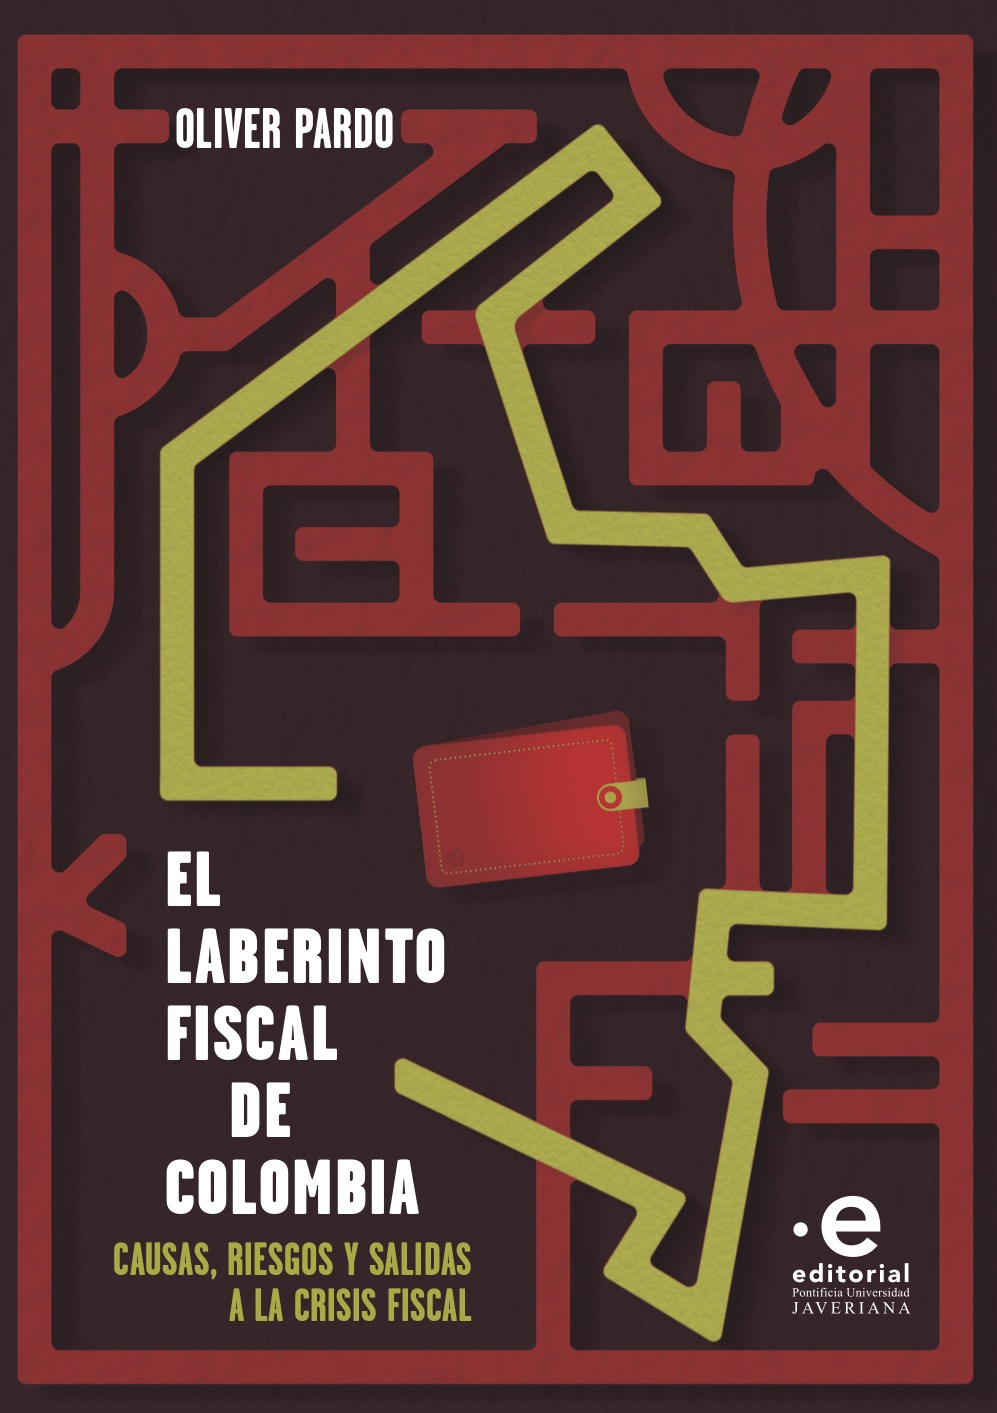
\includegraphics[width=\linewidth]{assets/laberinto_fiscal_portada.jpg}\\[-0.05cm]
    \tiny Editorial Javeriana, 2025
  \end{column}
\end{columns}
\note{[Sources] ProgramaFPC, Google Doc suministrado por el usuario, consultado el 29 de julio de 2026. Portada: Editorial Pontificia Universidad Javeriana, \href{https://www.javeriana.edu.co/web/editorial/w/laberinto-fiscal-colombia}{El laberinto fiscal de Colombia}.}
\end{frame}

\begin{frame}{M3: las reglas conectan el presupuesto con la sostenibilidad}
\footnotesize
\begin{block}{Lecturas obligatorias}
  \begin{itemize}
    \item L\'opez Velandia y L\'opez Ghio (2019), \textit{Regla fiscal para el gobierno central en Colombia}.
    \item FMI (2022), \textit{Fiscal Rules and Fiscal Councils: Recent Trends and Performance during the COVID-19 Pandemic}.
  \end{itemize}
\end{block}
\begin{block}{Lecturas sugeridas}
  \begin{itemize}
    \item Ministerio de Hacienda: MFMP 2026 e informe de cumplimiento de la regla fiscal 2025.
    \item Observatorio Fiscal PUJ: \textit{As\'i funciona el Presupuesto General de la Naci\'on}.
    \item Pardo (2025), \textit{El Laberinto Fiscal de Colombia}, cap. 3.
  \end{itemize}
\end{block}
\begin{alertblock}{Aplicaci\'on}
Herramienta PEPE: Presupuesto en Perspectiva Econ\'omica, Observatorio Fiscal PUJ.
\end{alertblock}
\note{[Sources] ProgramaFPC, Google Doc suministrado por el usuario, consultado el 29 de julio de 2026.}
\end{frame}

\begin{frame}{M4--M5: la seguridad social tambi\'en es pol\'itica fiscal}
\scriptsize
\begin{columns}[T,onlytextwidth]
  \begin{column}{0.49\textwidth}
    \begin{block}{M4. Pensiones}
      \textbf{Lecturas obligatorias}
      \begin{itemize}
        \item Observatorio Fiscal PUJ, \textit{Gu\'ia Ciudadana al Sistema de Pensiones y la Protecci\'on de la Vejez}.
        \item Observatorio Fiscal PUJ, \textit{Primer an\'alisis del Proyecto de Reforma Pensional}.
        \item Hartmann y Pardo, \textit{C\'omo financiar el Pilar Solidario sin reventar el Presupuesto}.
      \end{itemize}
      \textbf{Datos:} introducci\'on y uso de la GEIH.
    \end{block}
  \end{column}
  \begin{column}{0.49\textwidth}
    \begin{block}{M5. Salud}
      \textbf{Lecturas obligatorias}
      \begin{itemize}
        \item Observatorio Fiscal PUJ, \textit{Gu\'ia Ciudadana al Sistema de Salud}.
        \item ACEMI (2026), propuestas para la estabilizaci\'on y fortalecimiento del sistema de salud 2026--2030.
      \end{itemize}
      \textbf{Datos:} introducci\'on y uso de SICODIS.
    \end{block}
  \end{column}
\end{columns}
\note{[Sources] ProgramaFPC, Google Doc suministrado por el usuario, consultado el 29 de julio de 2026.}
\end{frame}

\begin{frame}{M6 y M7: territorio y comparaci\'on internacional}
\scriptsize
\begin{columns}[T,onlytextwidth]
  \begin{column}{0.57\textwidth}
    \begin{block}{M6. Finanzas p\'ublicas territoriales}
      \textbf{Obligatorias}
      \begin{itemize}
        \item Observatorio Fiscal PUJ, \textit{¿De d\'onde vienen y hacia d\'onde van los recursos de mi municipio?}
        \item Comisi\'on de Estudio del Sistema Tributario Territorial (2020), \textit{Informe Final}.
      \end{itemize}
      \textbf{Sugeridas}
      \begin{itemize}
        \item Carreri y Martinez (2023), reglas fiscales y rendici\'on de cuentas.
        \item \textit{A subnational resource curse?}
      \end{itemize}
      \textbf{Datos:} Terridata y FUT.
    \end{block}
  \end{column}
  \begin{column}{0.40\textwidth}
    \begin{block}{M7. Contexto internacional}
      \textbf{Lectura obligatoria}\\[0.15cm]
      FMI, \textit{Colombia: 2024 Article IV Consultation---Staff Report}.
    \end{block}
    \begin{alertblock}{Pregunta transversal}
      ¿En qu\'e se parece y en qu\'e se diferencia Colombia de otras econom\'ias comparables?
    \end{alertblock}
  \end{column}
\end{columns}
\note{[Sources] ProgramaFPC, Google Doc suministrado por el usuario, consultado el 29 de julio de 2026.}
\end{frame}

\begin{frame}{M8: la presentaci\'on debe conducir a una discusi\'on}
\small
\begin{block}{Formato}
  Grupos de 2--3 estudiantes. La sesi\'on puede durar hasta dos horas y debe reservar al menos una hora para discusi\'on.
\end{block}
\begin{columns}[T,onlytextwidth]
  \begin{column}{0.48\textwidth}
    \begin{itemize}
      \item Crisis fiscal
      \item Crisis del sistema de salud
      \item Reforma pensional
      \item Cajas de compensaci\'on
      \item Ecopetrol
    \end{itemize}
  \end{column}
  \begin{column}{0.48\textwidth}
    \begin{itemize}
      \item Pol\'itica monetaria y dominancia fiscal
      \item Finanzas de una entidad territorial
      \item Renta de personas jur\'idicas
      \item Renta de personas naturales
      \item Reforma al IVA
    \end{itemize}
  \end{column}
\end{columns}
\note{[Sources] ProgramaFPC, Google Doc suministrado por el usuario, consultado el 29 de julio de 2026.}
\end{frame}

\begin{frame}{M8: coyuntura, presupuesto y territorio}
\small
\begin{columns}[T,onlytextwidth]
  \begin{column}{0.48\textwidth}
    \begin{itemize}
      \item Ejecuci\'on del PGN 2025
      \item PGN 2026
      \item PGN 2027
      \item MFMP 2026
      \item Ejecuci\'on del presupuesto de regal\'ias 2023--2024
    \end{itemize}
  \end{column}
  \begin{column}{0.48\textwidth}
    \begin{itemize}
      \item Formulaci\'on del presupuesto de regal\'ias 2025--2026
      \item Art\'iculo IV del FMI
      \item Catastro multiprop\'osito
      \item Activaci\'on de la cl\'ausula de escape
      \item Otro tema fiscal acordado con el profesor
    \end{itemize}
  \end{column}
\end{columns}
\begin{alertblock}{Criterio}
El listado no es exhaustivo: un grupo puede proponer otro tema y solicitar referencias al profesor.
\end{alertblock}
\note{[Sources] ProgramaFPC, Google Doc suministrado por el usuario, consultado el 29 de julio de 2026.}
\end{frame}

\begin{frame}
  \frametitle{Funciones del Estado y su Base Constitucional}
  \begin{itemize}
    \item \textbf{Legislativa:} Crear leyes (Art. 1, 3)
    \item \textbf{Ejecutiva:} Administrar y ejecutar leyes (Art. 113, 209)
    \item \textbf{Judicial:} Aplicar justicia (Art. 229, 228)
    \item \textbf{Defensa y seguridad:} Proteger soberan\'ia y orden (Art. 2)
    \item \textbf{Econ\'omica:} Dirigir la econom\'ia y corregir desigualdades (Art. 1, 334)
    \item \textbf{Social:} Garantizar derechos b\'asicos (Art. 1, 2, 366)
    \item \textbf{Fiscal:} Recaudar y asignar recursos (Art. 338, 95)
    \item \textbf{Reguladora:} Supervisar mercados y servicios (Art. 333, 365)
  \end{itemize}
\end{frame}

\begin{frame}
  \frametitle{Art\'iculo 1 - CP de 1991}
  Colombia es un Estado social de derecho, organizado en forma de Rep\'ublica unitaria, descentralizada, con autonom\'ia de sus entidades territoriales, democr\'atica, participativa y pluralista, fundada en el respeto de la dignidad humana, en el trabajo y la solidaridad de las personas que la integran y en la prevalencia del inter\'es general.
\end{frame}

\begin{frame}
  \frametitle{Art\'iculo 2 - CP de 1991}
  Son fines esenciales del Estado: servir a la comunidad, promover la prosperidad general y garantizar la efectividad de los principios, derechos y deberes consagrados en la Constituci\'on; facilitar la participaci\'on de todos en las decisiones que los afectan y en la vida econ\'omica, pol\'itica, administrativa y cultural de la Naci\'on; defender la independencia nacional, mantener la integridad territorial y asegurar la convivencia pac\'ifica y la vigencia de un orden justo.
\end{frame}

\begin{frame}
  \frametitle{Art\'iculo 3 - CP de 1991}
  La soberan\'ia reside exclusivamente en el pueblo, del cual emana el poder p\'ublico. El pueblo la ejerce en forma directa o por medio de sus representantes, en los t\'erminos que la Constituci\'on establece.
\end{frame}

\begin{frame}
  \frametitle{Art\'iculo 95 - CP de 1991}
  La constituci\'on establece como deber de la persona y del ciudadano contribuir al financiamiento de los gastos e inversiones del Estado dentro de conceptos de justicia y equidad.
\end{frame}

\begin{frame}
  \frametitle{Art\'iculo 113 - CP de 1991}
  Son ramas del poder p\'ublico la legislativa, la ejecutiva y la judicial. Adem\'as de los \'organos que las integran, existen otros, aut\'onomos e independientes, para el cumplimiento de las funciones del Estado. Los diferentes \'organos del Estado tienen funciones separadas pero colaboran arm\'onicamente para la realizaci\'on de sus fines.
\end{frame}

\begin{frame}{El Estado es m\'as amplio que las tres ramas}
\scriptsize
\begin{columns}[T,onlytextwidth]
  \begin{column}{0.32\textwidth}
    \begin{block}{Rama legislativa}
      \textbf{Congreso de la Rep\'ublica}
      \begin{itemize}
        \item Senado
        \item C\'amara de Representantes
      \end{itemize}
      Hace las leyes, reforma la Constituci\'on y ejerce control pol\'itico.
    \end{block}
  \end{column}
  \begin{column}{0.32\textwidth}
    \begin{block}{Rama ejecutiva}
      \textbf{Orden nacional}
      \begin{itemize}
        \item Presidencia
        \item Sectores (Hacienda, Defensa, Salud, etc)
      \end{itemize}
      \textbf{Orden territorial:} Gobernaciones y Alcald\'ias.
    \end{block}
  \end{column}
  \begin{column}{0.32\textwidth}
    \begin{block}{Rama judicial}
      \begin{itemize}
        \item Corte Constitucional
        \item Corte Suprema 
        %\item Consejo de Estado
        \item Fiscal\'ia General
        \item Tribunales y juzgados
        %\item Gobierno y disciplina judicial
      \end{itemize}
    \end{block}
  \end{column}
\end{columns}
\vspace{0.15cm}
\begin{alertblock}{Organismos autónomos}
 Contralor\'ia y Procuraduría.
\quad  CNE y Registradur\'ia.
\quad Banco de la Rep\'ublica.
\end{alertblock}
\note{[Sources] Constituci\'on Pol\'itica de Colombia, arts. 113--120, 249, 265--266, 267, 275, 371 y 130. Texto oficial: Secretar\'ia del Senado.}
\end{frame}

\begin{frame}{La separaci\'on es funcional, no aislamiento}
\small
\begin{tabular}{p{0.19\textwidth}p{0.36\textwidth}p{0.36\textwidth}}
\textbf{Rama} & \textbf{Funci\'on principal} & \textbf{Ejemplo fiscal} \\ \hline
\textbf{Legislativa} &
Expide leyes, reforma la Constituci\'on y controla pol\'iticamente al Gobierno. &
Aprueba tributos, presupuesto y endeudamiento dentro de sus competencias. \\[0.18cm]
\textbf{Ejecutiva} &
Formula pol\'iticas, administra y reglamenta las leyes sin sustituir al legislador. &
Presenta el presupuesto, recauda, ejecuta el gasto y expide decretos reglamentarios. \\[0.18cm]
\textbf{Judicial} &
Resuelve controversias y controla la constitucionalidad o legalidad seg\'un la jurisdicci\'on. &
Puede retirar o suspender normas fiscales incompatibles con normas superiores. \\
\end{tabular}
\vspace{0.25cm}
\begin{block}{Regla de lectura}
Las funciones est\'an separadas, pero los \'organos colaboran arm\'onicamente y se controlan entre s\'i. La competencia concreta siempre depende de la Constituci\'on y la ley. En la práctica, habrán controversias.
\end{block}
\note{[Sources] Constituci\'on Pol\'itica, arts. 113--116, 150, 189, 241 y 237.}
\end{frame}

\begin{frame}{Jerarqu\'ia normativa: qui\'en expide y qui\'en modifica}
\scriptsize
\begin{tabular}{p{0.22\textwidth}p{0.31\textwidth}p{0.38\textwidth}}
\textbf{Nivel} & \textbf{Qui\'en la expide} & \textbf{C\'omo se modifica o controla} \\ \hline
\textbf{Constituci\'on} &
Pueblo constituyente; Congreso mediante acto legislativo. &
Acto legislativo, referendo o asamblea constituyente. La Corte controla los procedimientos de reforma. \\[0.16cm]
\textbf{Leyes} &
Congreso; el Presidente sanciona y promulga. &
Otra ley del tipo y tr\'amite exigidos. La Corte Constitucional puede declarar su inexequibilidad. \\[0.16cm]
\textbf{Decretos con fuerza de ley} &
Gobierno por habilitaci\'on constitucional: facultades extraordinarias o estados de excepci\'on. &
El Congreso puede modificarlos por ley dentro de sus competencias; la Corte controla sus l\'imites de materia, tiempo y procedimiento. \\[0.16cm]
\textbf{Decretos reglamentarios} &
Presidente y Gobierno para ejecutar la ley. &
No pueden crear ni modificar la ley. El Gobierno puede derogarlos y la jurisdicci\'on contenciosa controla su legalidad. \\[0.16cm]
\textbf{Actos administrativos} &
Ministros y otras autoridades: resoluciones, circulares y \'ordenes, seg\'un competencia. &
Deben respetar Constituci\'on, ley y reglamentos superiores; pueden ser revocados o anulados conforme al ordenamiento. \\
\end{tabular}
\vspace{0.12cm}
%\textit{Precisi\'on:} no existe una pir\'amide exhaustiva y lineal para todas las normas. Importan tambi\'en la materia, la competencia y los procedimientos especiales.
\note{[Sources] Constituci\'on Pol\'itica, arts. 4, 150, 189.10--11, 212--215, 241 y 374--379; Corte Constitucional, sentencias C-037 de 2000 y C-536 de 2005.}
\end{frame}

%\begin{frame}{Los contrapesos operan antes y despu\'es de decidir}
%\small
%\begin{tikzpicture}[
%  node distance=1.3cm and 1.5cm,
%  organ/.style={rectangle, rounded corners, draw=blue!70, fill=blue!8,
%    text width=3.0cm, minimum height=1.05cm, align=center},
%  control/.style={-{Stealth[length=2mm]}, thick, draw=black!65}
%]
%  \node[organ] (congreso) {\textbf{Congreso}\\leyes, presupuesto\\y control pol\'itico};
%  \node[organ, right=of congreso] (gobierno) {\textbf{Gobierno}\\sanci\'on u objeci\'on\\y ejecuci\'on};
%  \node[organ, below=of congreso] (corte) {\textbf{Corte Constitucional}\\control de la ley y de\\decretos con fuerza de ley};
%  \node[organ, right=of corte] (consejo) {\textbf{Consejo de Estado}\\control de actos\\administrativos};

%  \draw[control, bend left=12] (congreso) to node[above, sloped, font=\tiny]{autoriza y controla} (gobierno);
%  \draw[control, bend left=12] (gobierno) to node[below, sloped, font=\tiny]{sanciona u objeta} (congreso);
%  \draw[control] (corte) -- node[left, font=\tiny]{constitucionalidad} (congreso);
%  \draw[control] (corte) -- node[below, sloped, font=\tiny]{l\'imites constitucionales} (gobierno);
%  \draw[control] (consejo) -- node[right, font=\tiny]{legalidad} (gobierno);
%\end{tikzpicture}
%\vspace{0.15cm}
%\begin{alertblock}{Controles transversales}
%Contralor\'ia: control fiscal. %Procuraduría: vigilancia disciplinaria y protecci\'on de derechos; 
%Ciudadan\'ia: voto, tutela y derechos de petición.
%\end{alertblock}
%\note{[Sources] Constituci\'on Pol\'itica, arts. 113, 135, 150, 167, 189, 237, 241, 267 y 275--282.}
%\end{frame}

\begin{frame}
  \frametitle{Art\'iculo 209 - CP de 1991}
  La funci\'on administrativa est\'a al servicio de los intereses generales y se desarrolla con fundamento en los principios de igualdad, moralidad, eficacia, econom\'ia, celeridad, imparcialidad y publicidad, mediante la descentralizaci\'on, la delegaci\'on y la desconcentraci\'on de funciones.
\end{frame}

\begin{frame}
  \frametitle{Art\'iculo 228 - CP de 1991}
  La administraci\'on de justicia es funci\'on p\'ublica. Sus decisiones son independientes. Las actuaciones ser\'an p\'ublicas y permanentes, con las excepciones que establezca la ley, y los t\'erminos procesales se observar\'an con diligencia. Su funcionamiento ser\'a desconcentrado y aut\'onomo.
\end{frame}

\begin{frame}
  \frametitle{Art\'iculo 229 - CP de 1991}
  Se garantiza el derecho de toda persona para acceder a la administraci\'on de justicia. La ley indicar\'a en qu\'e casos puede hacerlo sin la representaci\'on de abogado.
\end{frame}

\begin{frame}
  \frametitle{Art\'iculo 333 - CP de 1991}
  La actividad econ\'omica y la iniciativa privada son libres, dentro de los l\'imites del bien com\'un. La empresa, como base del desarrollo, tiene una funci\'on social que implica obligaciones. El Estado, por mandato de la ley, intervendr\'a por razones de utilidad p\'ublica o de inter\'es social.
\end{frame}

\begin{frame}
  \frametitle{Art\'iculo 334 - CP de 1991}
  El Estado intervendr\'a por mandato de la ley en la explotaci\'on de los recursos naturales, en el uso del suelo, en la producci\'on, distribuci\'on, utilizaci\'on y consumo de los bienes, y en los servicios p\'ublicos y privados, para racionalizar la econom\'ia con el fin de conseguir el mejoramiento de la calidad de vida.
\end{frame}

\begin{frame}
  \frametitle{Art\'iculo 338 - CP de 1991}
  En tiempo de paz, solamente el Congreso, las asambleas departamentales y los concejos distritales y municipales podr\'an imponer contribuciones fiscales o parafiscales. La ley, las ordenanzas y los acuerdos deben fijar directamente los sujetos activos y pasivos, los hechos y las bases gravables, y las tarifas de los impuestos.
\end{frame}

\begin{frame}
  \frametitle{Art\'iculo 365 - CP de 1991}
  Los servicios p\'ublicos son inherentes a la finalidad social del Estado. Es deber del Estado asegurar su prestaci\'on eficiente a todos los habitantes del territorio nacional. Podr\'an ser prestados por el Estado, directa o indirectamente, por comunidades organizadas, o por particulares.
\end{frame}

\begin{frame}
  \frametitle{Art\'iculo 366 - CP de 1991}
  El bienestar general y el mejoramiento de la calidad de vida de la poblaci\'on son finalidades sociales del Estado. Ser\'a objetivo fundamental de su actividad la soluci\'on de las necesidades insatisfechas de salud, de educaci\'on, de saneamiento ambiental y de agua potable.
\end{frame}


\begin{frame}
  \frametitle{Funciones del Estado y su Base Constitucional}
  \begin{itemize}
    \item \textbf{Legislativa:} Crear leyes (Art. 1, 3)
    \item \textbf{Ejecutiva:} Administrar y ejecutar leyes (Art. 113, 209)
    \item \textbf{Judicial:} Aplicar justicia (Art. 229, 228)
    \item \textbf{Defensa y seguridad:} Proteger soberan\'ia y orden (Art. 2)
    \item \textbf{Econ\'omica:} Dirigir la econom\'ia y corregir desigualdades (Art. 1, 334)
    \item \textbf{Social:} Garantizar derechos b\'asicos (Art. 1, 2, 366)
    \item \textbf{Fiscal:} Recaudar y asignar recursos (Art. 338, 95)
    \item \textbf{Reguladora:} Supervisar mercados y servicios (Art. 333, 365)
  \end{itemize}
\end{frame}

\begin{frame}{Desagregaci\'on del Sector P\'ublico Consolidado}
\centering
\begin{tikzpicture}[node distance=0.5cm and 0.5cm, every node/.style={align=center},
  box/.style={rectangle, draw, rounded corners, text width=3cm, minimum height=0.7cm},
  level/.style={rectangle, draw, text width=3cm, minimum height=0.7cm}]

\node[box, fill=blue!10] (spc) {\tiny{Sector P\'ublico Consolidado}};

\node[level, below left=of spc] (spf) {\tiny{Sector Público Financiero}};
\node[level, fill=green!10, below =of spc] (spnf) {\tiny{Sector Público No Financiero}};


\node[level, fill=green!10, below=of spnf] (gg) {\tiny{Gobierno General}};
\node[level, below left =of spnf] (eepp) {\tiny{Empresas Públicas}};


\node[level, fill=red!10, below left=of gg] (gnc) {\tiny{Gobierno Nacional Central}};
\node[level, fill=red!10, below =of gg] (et) {\tiny{Entidades Territoriales}};
\node[level, fill=red!10, below right =of gg] (ss) {\tiny{Seguridad Social}};

%\node[level, below left=of ss] (salud) {\tiny{Salud}};
%\node[level, below right =of ss] (pensiones) {\tiny{Pensiones}};

\node[box, fill=blue!10] (spc) {Sector P\'ublico Consolidado};

% Conexiones directas desde SPC
\draw[->] (spc) -- (spf);
\draw[->] (spc) -- (spnf);

\draw[->] (spnf) -- (gg);
\draw[->] (spnf) -- (eepp);

\draw[->] (gg) -- (gnc);
\draw[->] (gg) -- (et);
\draw[->] (gg) -- (ss);
\end{tikzpicture}
\end{frame}




\section{Sector público y contabilidad fiscal}
\begin{frame}{Desagregaci\'on del Sector P\'ublico Consolidado}
\centering
\begin{tikzpicture}[node distance=0.5cm and 0.5cm, every node/.style={align=center},
  box/.style={rectangle, draw, rounded corners, text width=3cm, minimum height=0.7cm},
  level/.style={rectangle, draw, text width=3cm, minimum height=0.7cm}]

\node[box, fill=blue!10] (spc) {\tiny{Sector P\'ublico Consolidado}};

\node[level, below left=of spc] (spf) {\tiny{Sector Público Financiero}};
\node[level, fill=green!10, below =of spc] (spnf) {\tiny{Sector Público No Financiero}};


\node[level, fill=green!10, below=of spnf] (gg) {\tiny{Gobierno General}};
\node[level, below left =of spnf] (eepp) {\tiny{Empresas Públicas}};


\node[level, fill=red!10, below left=of gg] (gnc) {\tiny{Gobierno Nacional Central}};
\node[level, fill=red!10, below =of gg] (et) {\tiny{Entidades Territoriales}};
\node[level, fill=red!10, below right =of gg] (ss) {\tiny{Seguridad Social}};

%\node[level, below left=of ss] (salud) {\tiny{Salud}};
%\node[level, below right =of ss] (pensiones) {\tiny{Pensiones}};

\node[box, fill=blue!10] (spc) {Sector P\'ublico Consolidado};

% Conexiones directas desde SPC
\draw[->] (spc) -- (spf);
\draw[->] (spc) -- (spnf);

\draw[->] (spnf) -- (gg);
\draw[->] (spnf) -- (eepp);

\draw[->] (gg) -- (gnc);
\draw[->] (gg) -- (et);
\draw[->] (gg) -- (ss);
\end{tikzpicture}
\end{frame}


\begin{frame}{Definición de balance en billones de pesos}
\begin{equation*}
B = T - G
\end{equation*}
\vspace{0.5em}
\begin{itemize}
  \item $B$: Balance fiscal en billones de pesos
  \item $T$: Ingresos totales del gobierno
  \item $G$: Gasto total del gobierno (incluye intereses)
\end{itemize}
\end{frame}

\begin{frame}{Relación entre déficit y balance}
\begin{equation*}
\text{Déficit} = -B
\end{equation*}
\vspace{0.5em}
\begin{itemize}
  \item $B$: Balance fiscal en billones de pesos
  \item Si $B < 0$, el gobierno tiene un déficit
  \item Si $B > 0$, el gobierno tiene un superávit
  %\item Por convención, el déficit es una magnitud positiva
\end{itemize}
\end{frame}


\begin{frame}{PIB de Colombia en 2026}
\begin{itemize}
  \item \textbf{PIB nominal proyectado de Colombia en 2026:} \\
  \quad \$1,998 billones de pesos corrientes
  
  \vspace{1em}
  \item \textbf{1 punto del PIB:} \\
  \quad \$1,998 billones × 1\% = \textbf{\$19.98 billones de pesos}
  
  \vspace{1em}
  \item Esta equivalencia permite interpretar los saldos fiscales expresados como porcentaje del PIB en términos absolutos.
\end{itemize}
\end{frame}


\begin{frame}{Definición de balance como porcentaje del PIB}
\begin{equation*}
b = t - g
\end{equation*}
\vspace{0.5em}
\begin{itemize}
  \item $b$: Balance fiscal como porcentaje del PIB
  \item $t$: Ingresos totales del gobierno
  \item $g$: Gasto total del gobierno (incluye intereses)
\end{itemize}
\end{frame}

\begin{frame}{Relación entre niveles y proporciones del PIB}
\begin{align*}
b &= \frac{B}{PIB} = \frac{T - G}{PIB} = \frac{T}{PIB} - \frac{G}{PIB} = t - g
\end{align*}
\vspace{0.5em}
\begin{itemize}
  \item $b$: Balance fiscal como \% del PIB
  \item $B$: Balance fiscal en billones de pesos
  \item $t = \frac{T}{PIB}$: Ingresos como \% del PIB
  \item $g = \frac{G}{PIB}$: Gasto como \% del PIB
\end{itemize}
\end{frame}

\begin{frame}{Desagregaci\'on del Sector P\'ublico Consolidado}
\centering
\begin{tikzpicture}[node distance=0.5cm and 0.5cm, every node/.style={align=center},
  box/.style={rectangle, draw, rounded corners, text width=3cm, minimum height=0.7cm},
  level/.style={rectangle, draw, text width=3cm, minimum height=0.7cm}]

\node[box, fill=blue!10] (spc) {\tiny{Sector P\'ublico Consolidado}};

\node[level, below left=of spc] (spf) {\tiny{Sector Público Financiero}};
\node[level, fill=green!10, below =of spc] (spnf) {\tiny{Sector Público No Financiero}};


\node[level, fill=green!10, below=of spnf] (gg) {\tiny{Gobierno General}};
\node[level, below left =of spnf] (eepp) {\tiny{Empresas Públicas}};


\node[level, fill=red!10, below left=of gg] (gnc) {\tiny{Gobierno Nacional Central}};
\node[level, fill=red!10, below =of gg] (et) {\tiny{Entidades Territoriales}};
\node[level, fill=red!10, below right =of gg] (ss) {\tiny{Seguridad Social}};

%\node[level, below left=of ss] (salud) {\tiny{Salud}};
%\node[level, below right =of ss] (pensiones) {\tiny{Pensiones}};

\node[box, fill=blue!10] (spc) {Sector P\'ublico Consolidado};

% Conexiones directas desde SPC
\draw[->] (spc) -- (spf);
\draw[->] (spc) -- (spnf);

\draw[->] (spnf) -- (gg);
\draw[->] (spnf) -- (eepp);

\draw[->] (gg) -- (gnc);
\draw[->] (gg) -- (et);
\draw[->] (gg) -- (ss);
\end{tikzpicture}
\end{frame}

\begin{frame}[t]{Balance fiscal del Sector Público No Financiero, 2025}

\vspace{-0.4em}

\begin{table}
\centering

{\small Balances por subsector (\% del PIB)}

\vspace{0.4em}

\fontsize{5.2}{5.9}\selectfont
\renewcommand{\arraystretch}{1.05}
\setlength{\tabcolsep}{2pt}

\begin{tabular}{
    @{}p{0.35\linewidth}r
    @{\hspace{6pt}}
    p{0.35\linewidth}r@{}
}

\hline
\textbf{Subsector} & \textbf{2025*}
& \textbf{Subsector} & \textbf{2025*} \\
\hline

\textbf{Sector Público No Financiero (SPNF)}
& \textbf{-6.7}
& Seguridad social
& 0.4
\\

\textbf{Gobierno General (GG)}
& \textbf{-6.1}
& \textbf{Empresas}
& \textbf{-0.2}
\\

\hspace{0.5em} Gobierno central
& -6.1
& \hspace{0.5em} Empresas nacionales
& 0.0
\\

\hspace{1em} Gobierno Nacional Central (GNC)
& -6.4
& \hspace{1em} Sector eléctrico
& 0.0
\\

\hspace{1em} Resto del Gobierno Central
& 0.2
& \hspace{1em} Ecopetrol
& 0.0
\\

\hspace{1.5em} Establecimientos públicos
& 0.0
& \hspace{1em} Telecom
& 0.0
\\

\hspace{1.5em} Agencia Nacional de Hidrocarburos (ANH)
& -0.1
& \hspace{0.5em} Empresas locales
& -0.2
\\

\hspace{1.5em} Fondo Nacional del Café (FNC)
& 0.0
& \hspace{1em} Empresas Públicas de Medellín (EPM)
& -0.2
\\

\hspace{1.5em} FEPC
& 0.2
& \hspace{1em} ETB
& 0.0
\\

\hspace{1.5em} Fondes
& 0.0
& \hspace{1em} Metro de Medellín
& 0.0
\\

\hspace{0.5em} Regionales y locales
& -0.4
& \hspace{1em} EAAB
& 0.0
\\

\hspace{1em} Administraciones centrales de las ET
& -0.2
& \hspace{1em} Empresas Municipales de Cali (Emcali)
& 0.0
\\

\hspace{1em} Sistema General de Regalías (SGR)
& -0.2
& \textbf{Sector Público No Modelado (SPNM)}
& \textbf{-0.4}
\\

\hspace{1em} Fondo de Ahorro y Estabilización Petrolera (FAEP)
& 0.0
& \textbf{Balance primario del SPNF}
& \textbf{-3.4}
\\

\hline

\end{tabular}

\end{table}

\vfill


\end{frame}

\begin{frame}{Definiciones: gasto primario y balance primario}
\begin{align*}
GP &= G - I \\
P &= T - GP = T - (G - I) = B + I
\end{align*}
\vspace{0.5em}
\begin{itemize}
  \item $GP$: Gasto primario en billones de pesos (excluye intereses)
  \item $G$: Gasto total del gobierno (incluye intereses)
  \item $I$: Pago de intereses en billones de pesos
  \item $P$: Balance primario en billones de pesos
  \item $T$: Ingresos totales del gobierno
  \item $B$: Balance fiscal total en billones de pesos
\end{itemize}
\end{frame}

\begin{frame}{Gasto primario y balance primario como \% del PIB}
\begin{align*}
gp &= g - i \\
p &= t - gp = t - (g - i) = b + i
\end{align*}
\vspace{0.5em}
\begin{itemize}
  \item $gp$: Gasto primario como porcentaje del PIB
  \item $g$: Gasto total del gobierno como \% del PIB
  \item $i$: Intereses como \% del PIB
  \item $p$: Balance primario como \% del PIB
  \item $t$: Ingresos totales como \% del PIB
  \item $b$: Balance fiscal total como \% del PIB
\end{itemize}
\end{frame}

\begin{frame}{Recordatorio contable: ¿Qué es el patrimonio?}
\begin{equation*}
\textbf{Patrimonio} = \text{Activos} - \text{Pasivos}
\end{equation*}

\vspace{1em}
\begin{itemize}
  \item \textbf{Activos:} Bienes y derechos que posee el Estado (efectivo, inversiones, infraestructura, cuentas por cobrar, etc.)
  \item \textbf{Pasivos:} Obligaciones del Estado (deuda pública, cuentas por pagar, etc.)
  \item \textbf{Patrimonio:} Es la diferencia entre lo que el Estado posee y lo que debe.
\end{itemize}

\vspace{1em}
\textit{El balance fiscal refleja el cambio en ese patrimonio, excluyendo operaciones que solo modifican activos y pasivos sin efecto patrimonial.}
\end{frame}


\begin{frame}{¿Por qué las amortizaciones no son gasto público?}
\textbf{El balance mide el cambio en el patrimonio :}
\begin{equation*}
\text{Balance} = \text{Ingresos} - \text{Gastos}
\end{equation*}

\vspace{1em}
\textbf{Implicación contable:}
\begin{itemize}
  \item Solo se incluyen operaciones que afectan el \textbf{patrimonio}.
  \item Las \textbf{amortizaciones} (pago del principal de la deuda) reducen un activo...
  \item ... pero también reducen un pasivo (deuda) en el mismo monto.
  \item Por lo tanto, no afectan el patrimonio.
  \item Como consecuencia, no se consideran gasto.
\end{itemize}
\end{frame}

\begin{frame}
\textbf{En cambio, los intereses sí son gasto:}
\begin{itemize}
  \item Son un pago por el uso de recursos prestados.
  \item Disminuyen el patrimonio neto sin reducir pasivos.
\end{itemize}
\end{frame}

\begin{frame}{Ejercicio: ¿Qué parte de mi cuota hipotecaria es gasto?}
\textbf{Pago mensual:} \$6 millones

\vspace{0.5em}
\begin{itemize}
  \item \$4 millones corresponden a \textbf{intereses} → \textbf{Gasto}
  \item \$2 millones corresponden a \textbf{amortización del capital} → \textbf{No es gasto}
\end{itemize}

\vspace{1em}
\textbf{Interpretación:}
\begin{itemize}
  \item Los intereses reducen mi efectivo disponible pero no reducen mi deuda → reducen mi patrimonio →se consideran gasto.
  \item La amortización reduce mi efectivo disponible (activo) pero también reduce mi deuda (pasivo) → no afecta patrimonio! → no es gasto 
\end{itemize}

\vspace{1em}
\textit{Lo mismo aplica para las cuentas fiscales del gobierno.}
\end{frame}

\begin{frame}{Ejercicio: ¿Vender mi apartamento es un ingreso?}
\textbf{Supongamos:} Vendo mi apartamento por \$500 millones.

\vspace{1em}
\begin{itemize}
  \item Aumenta mi \textbf{activo líquido} (efectivo) en \$500 millones.
  \item Disminuye mi \textbf{activo fijo} (apartamento) en \$500 millones.
  \item \textbf{No cambia mi patrimonio neto.}
\end{itemize}

\vspace{1em}
\textbf{Conclusión:} No es un ingreso económico.  
Es una \textbf{reorganización de activos}, no un aumento de riqueza.

\vspace{1em}
\textit{En contabilidad pública, vender un activo (como una propiedad del Estado) no \textbf{debería} registrarse como ingreso fiscal.}
\end{frame}

\begin{frame}{Ejercicio: ¿Pedir prestado dinero es un ingreso?}
\textbf{Supongamos:} Pido prestados \$100 millones a un banco.

\vspace{1em}
\begin{itemize}
  \item Mi \textbf{activo} (efectivo disponible) aumenta en \$100 millones.
  \item Mi \textbf{pasivo} (deuda con el banco) también aumenta en \$100 millones.
  \item \textbf{No cambia mi patrimonio neto}.
\end{itemize}

\vspace{1em}
\textbf{Conclusión:}
\begin{itemize}
  \item No es un ingreso real.
  \item Es una \textbf{operación financiera}: financia mis gastos, pero no me vuelve más rico.
\end{itemize}

\vspace{1em}
\textit{Lo mismo aplica en las finanzas públicas: el endeudamiento no es ingreso fiscal.}
\end{frame}

\begin{frame}{Ejercicio: ¿La venta de ISA fue un ingreso fiscal?}
\textbf{En 2021, el Gobierno vendió su participación en ISA por \$14,2 billones.}

\vspace{1em}
\begin{itemize}
  \item Se redujo un \textbf{activo financiero} del Estado (participación accionaria en ISA).
  \item Se incrementó el \textbf{efectivo disponible} (activo líquido).
  \item \textbf{No cambió el patrimonio neto}: solo se intercambió un activo por otro.
\end{itemize}

\vspace{1em}
\textbf{Conclusión:}  
\begin{itemize}
  \item No fue un ingreso fiscal corriente.
  \item Se registró como una \textbf{fuente de financiamiento}, no como ingreso que mejora el balance fiscal.
\end{itemize}

\vspace{1em}
\textit{La venta de activos públicos no debe confundirse con un aumento permanente en los ingresos del gobierno.}
\end{frame}

\begin{frame}{Ingresos del GNC \$ MM}
\begin{center}
\adjustbox{max width=0.99\textwidth}{
  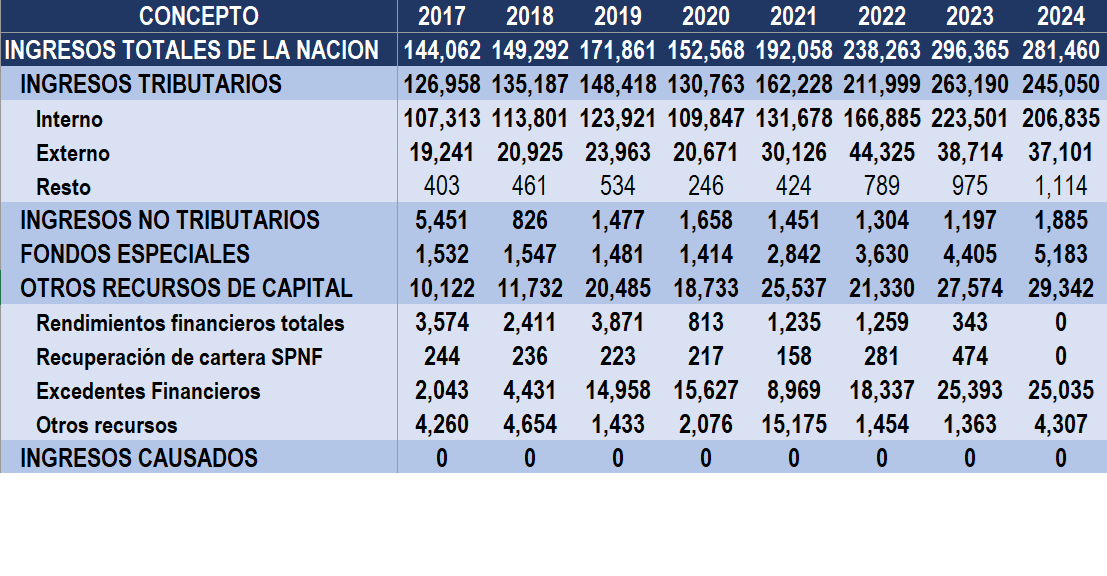
\includegraphics{assets/IngresosGNC.png}
}
\end{center}
\end{frame}



\begin{frame}{Pero el Gobierno hizo trampa...}
\textbf{¿Qué pasó realmente con la venta de ISA?}

\vspace{1em}
\begin{itemize}
  \item Aunque la operación fue una \textbf{enajenación de activos}, el Gobierno la registró como un \textbf{ingreso de capital}.
  \item Esto permitió mostrar un \textbf{mejor balance fiscal} en 2021.
  \item La operación no correspondía a una fuente estructural ni a un ingreso tributario.
  \item Fue una forma de \textbf{mejorar artificialmente} el resultado fiscal, sin mejorar la sostenibilidad de largo plazo.
\end{itemize}

\vspace{1em}
\textit{Contablemente cuestionable, fiscalmente riesgoso.}
\end{frame}

\begin{frame}{Contabilidad presupuestal vs. contabilidad fiscal en Colombia}
\textbf{En Colombia, la contabilidad presupuestal y la contabilidad fiscal no coinciden.}

\vspace{1em}
\textbf{Contabilidad presupuestal:}
\begin{itemize}
  \item Se basa en el \textbf{Presupuesto General de la Nación (PGN)}.
  %\item Registra compromisos y apropiaciones aprobadas.
  \item Clasifica el gasto según \textbf{funcionamiento}, \textbf{inversión} y \textbf{servicio de la deuda}.
  \item Es una contabilidad jurídica y operativa.
\end{itemize}

\vspace{1em}
\textbf{Contabilidad fiscal:}
\begin{itemize}
  \item Sigue criterios del \textbf{Manual de Estadísticas de Finanzas Públicas (MEFP)} del FMI.
  \item Se enfoca en el  \textbf{cambio en el patrimonio}.
  \item (En teoría) excluye operaciones financieras como amortizaciones, prestamos o enajenación de activos.
\end{itemize}

\end{frame}





\section{Ciclo presupuestal}
\begin{frame}{¿Qué son las apropiaciones?}
\textbf{Apropiaciones:} son los \textbf{montos máximos autorizados por la Ley de Presupuesto} para ser comprometidos y ejecutados por una entidad pública.

\vspace{1em}
\begin{itemize}
  \item Representan el límite legal de gasto por cada rubro presupuestal.
  \item No implican ejecución automática ni gasto efectivo.
  \item Solo el Congreso puede modificarlas.
\end{itemize}

\vspace{1em}
\textit{Son el punto de partida del ciclo presupuestal.}
\end{frame}

\begin{frame}{¿Qué son los compromisos?}
\textbf{Compromisos:} son actos administrativos que generan una obligación futura de pago por parte del Estado.

\vspace{1em}
\begin{itemize}
  \item Se generan al contratar o adquirir bienes y servicios.
  \item Disminuyen el saldo disponible de la apropiación.
  \item Aún no son pagos, pero sí obligaciones asumidas formalmente.
\end{itemize}

\vspace{1em}
\textit{Ejemplo: firma de contrato de obra pública.}
\end{frame}

\begin{frame}{¿Qué son las obligaciones?}
\textbf{Obligaciones:} son los montos reconocidos como deuda cierta, exigible y cuantificada a favor de un tercero.

\vspace{1em}
\begin{itemize}
  \item Surgen cuando el bien o servicio ha sido entregado o prestado.
  \item Se sustentan con factura o documento equivalente.
  \item Deben pagarse dentro de los plazos legales.
\end{itemize}

\vspace{1em}
\textit{Ejemplo: recepción de una obra terminada.}
\end{frame}

\begin{frame}{¿Qué son los pagos?}
\textbf{Pagos:} son las erogaciones efectivas de recursos públicos para cumplir con obligaciones previamente reconocidas.

\vspace{1em}
\begin{itemize}
  \item Representan el último paso del ciclo presupuestal.
  \item Requieren disponibilidad de caja (tesorería).
  \item Pueden realizarse en el mismo año o en vigencias futuras.
\end{itemize}

\vspace{1em}
\textit{Ejemplo: giro de fondos al contratista.}
\end{frame}

\begin{frame}{Ciclo de ejecución presupuestal en Colombia}
\begin{center}
\begin{tikzpicture}[
  node distance=0.7cm,
  every node/.style={draw, rectangle, rounded corners, minimum width=3.8cm, minimum height=1cm, align=center},
  arrow/.style={->, thick}
]

\node (apropiacion) {Apropiación\\(autorización legal de gasto)};
\node (compromiso) [below=of apropiacion] {Compromiso\\(acto administrativo que genera obligación)};
\node (obligacion) [below=of compromiso] {Obligación\\(reconocimiento de deuda exigible)};
\node (pago) [below=of obligacion] {Pago\\(salida efectiva de recursos)};

\draw[arrow] (apropiacion) -- (compromiso);
\draw[arrow] (compromiso) -- (obligacion);
\draw[arrow] (obligacion) -- (pago);

\end{tikzpicture}
\end{center}
\end{frame}


\begin{frame}{Ciclo de ejecución presupuestal en Colombia}
\vspace{1em}
\begin{itemize}
  \item El ciclo puede abarcar más de una vigencia fiscal.
  \item Solo los pagos generan una salida de caja efectiva.
  \item En general, solo se considere como gasto cuando los recursos son \textbf{obligados}
\end{itemize}
\end{frame}

\begin{frame}{¿Qué es la ejecución presupuestal?}
\textbf{Ejecución presupuestal:} es el grado en que las apropiaciones autorizadas en el presupuesto se convierten en obligaciones durante el año fiscal.

\vspace{1em}
\begin{itemize}
  \item Mide cuánto del presupuesto aprobado va a ser irreversiblemente gastado.
  \item Se expresa usualmente como el porcentaje de obligaciones frente a apropiaciones.
\end{itemize}

\vspace{1em}
\textbf{Fórmula común:}
\begin{equation*}
\text{Ejecución (\%)} = \frac{\text{Obligaciones}}{\text{Apropiaciones}} \times 100
\end{equation*}

\vspace{1em}
\textit{Una alta ejecución no siempre implica buena calidad del gasto.}
\end{frame}

\begin{frame}{¿Qué pasa si una apropiación no se compromete en la vigencia?}
\begin{itemize}
  \item Las \textbf{apropiaciones} son válidas solo durante la vigencia fiscal (normalmente un año).
  \item Si al cierre de la vigencia una apropiación \textbf{no se compromete}, esa parte del presupuesto \textbf{se pierde} (pérdida de apropiación).
  \item En consecuencia, los recursos \textbf{no comprometidos se liberan o se cancelan} y se pierde la posibilidad de uso.
\end{itemize}
\end{frame}

\begin{frame}{¿Qué pasa si un compromiso no se obliga en la vigencia?}
\begin{itemize}
  \item Si existe un \textbf{compromiso registrado pero no obligado}, puede convertirse en \textbf{reserva presupuestal}.
  \item La reserva permite hacer el pago en el año siguiente, siempre que se haya comprometido oportunamente.
\end{itemize}
\end{frame}

\begin{frame}
\textbf{En resumen:}
\vspace{1em}
\begin{itemize}
  \item \textbf{Apropiación no comprometido} → se pierde.
  \item \textbf{Compromiso no obligado} → se convierte en \textbf{reserva presupuestal}.
\end{itemize}
\end{frame}



\begin{frame}
\vspace{1em}
\textbf{Implicaciones:}
\begin{itemize}
  \item Las entidades buscan alcanzar a al menos comprometer los recursos para no perderlos.
  \item Desde el punto de vista del cierre fiscal de la vigencia, una menor ejecución (las apropiaciones no alcanzan a obligarse) representa una mejora en el balance fiscal (aunque las reservas representan mayor presión fiscal para la vigencia siguiente).
  \item El retraso en los pagos facilita el manejo de caja.   
\end{itemize}

\end{frame}

\begin{frame}{Organigrama simplificado del Ministerio de Hacienda}
\begin{center}
\begin{tikzpicture}[
  every node/.style={rectangle, draw, align=center, rounded corners, font=\scriptsize, minimum width=3.2cm, minimum height=0.8cm},
  node distance=0.6cm
]

% Nivel 1
\node (ministro) {Ministro de Hacienda};

% Nivel 2
\node[below left=1.2cm and 1.2cm of ministro] (vicgen) {Viceministerio\\General};
\node[below right=1.2cm and 1.2cm of ministro] (victec) {Viceministerio\\Técnico};

% Nivel 3 - General
\node[below=of vicgen] (dgp) {DGPPN\\Presupuesto};
\node[below=of dgp] (dgcptn) {DGCPTN\\Crédito y Tesoro};
\node[below=of dgcptn] (dgaf) {DGAF\\Apoyo Fiscal};

% Nivel 3 - Técnico
\node[below=of victec] (polmacro) {DGPM \\ Política \\ Macroeconómica};
\node[below=of polmacro] (dgrees) {DGRESS\\Seguridad Social};

% Conexiones
\draw[->] (ministro) -- (vicgen);
\draw[->] (ministro) -- (victec);

\draw[->] (vicgen) -- (dgp);
\draw[->] (dgp) -- (dgcptn);
\draw[->] (dgcptn) -- (dgaf);

\draw[->] (victec) -- (polmacro);
\draw[->] (polmacro) -- (dgrees);

\end{tikzpicture}
\end{center}
\end{frame}





\section{Antecedentes macrofiscales}
\begin{frame}{}
\centering

\includegraphics[width=0.92\textwidth,height=0.86\textheight,keepaspectratio]{graficas/Cover.jpg}
%
\includegraphics[scale=0.5]{graficas/QR.jpeg}
\end{frame}

\input{slides/presentacion.tex}
\begin{frame}{El PIB real de 2025 superó en 16,1\% el nivel de 2019}
\centering
\begin{tikzpicture}
\begin{axis}[
    width=12cm,
    height=6.8cm,
    ylabel={PIB real (2019=1)},
    xtick={2019,2020,2021,2022,2023,2024,2025},
    xticklabel style={rotate=45,anchor=east},
    ymin=0.90,
    ymax=1.20,
    grid=both,
    grid style=dashed,
    thick
]
\addplot[color=blue,mark=*,very thick] coordinates {
    (2019,1.0000)
    (2020,0.9281)
    (2021,1.0284)
    (2022,1.1033)
    (2023,1.1101)
    (2024,1.1312)
    (2025,1.1606)
};
\end{axis}
\end{tikzpicture}
\vspace{0.15cm}
\scriptsize Fuente: DANE y MFMP 2026, tabla 1.2. Para 2025 se aplica el crecimiento real de 2,6\% reportado por el MFMP al nivel de 2024.
\note{[Sources] MFMP 2026, capítulo 1, tabla 1.2. Serie 2019-2024: DANE, como en la versión fuente.}
\end{frame}
\begin{frame}{El gasto primario alcanzó 19,9\% del PIB en 2025}
\centering
\resizebox{0.90\textwidth}{!}{
\begin{tikzpicture}
\begin{axis}[
    width=16.5cm,
    height=9cm,
    ylabel={\% del PIB},
    xtick={7,8,...,22},
    xticklabels={2011,2012,2013,2014,2015,2016,2017,2018,2019,2020,2021,2022,2023,2024,2025,2026},
    x tick label style={rotate=90,anchor=east},
    ymin=14,
    ymax=25,
    grid=both,
    grid style=dashed,
    legend style={at={(0.5,1.02)},anchor=south,legend columns=-1}
]
\addplot[color=blue,mark=*,very thick] coordinates {
    (7,15.3) (8,15.8) (9,16.8) (10,16.7) (11,16.5) (12,16.0)
    (13,16.4) (14,15.4) (15,15.8) (16,20.2) (17,19.8) (18,17.2)
    (19,19.1) (20,18.8) (21,19.9)
};
\addlegendentry{Gasto primario}
\addplot[color=red,mark=square*,very thick] coordinates {
    (7,18.0) (8,18.4) (9,19.1) (10,18.9) (11,19.1) (12,18.9)
    (13,19.3) (14,18.2) (15,18.7) (16,23.1) (17,23.1) (18,21.5)
    (19,22.9) (20,23.1) (21,22.7)
};
\addlegendentry{Gasto total}
\addplot[color=blue!60!black,dashed,thick] coordinates {(21,19.9) (22,18.2)};
\addplot[color=red!60!black,dashed,thick] coordinates {(21,22.7) (22,21.4)};
\addplot[color=gray,mark=*,only marks] coordinates {(22,18.2)};
\addplot[color=gray,mark=square*,only marks] coordinates {(22,21.4)};
\end{axis}
\end{tikzpicture}}
\scriptsize Línea sólida: resultados observados hasta 2025. Línea discontinua: proyección 2026.
\note{[Sources] MFMP 2026, capítulo 1, tablas 1.3 y 1.5. Serie histórica previa: MHCP, como en la versión fuente.}
\end{frame}
\begin{frame}{Los ingresos tributarios aumentaron a 14,7\% del PIB en 2025}
\centering
\resizebox{0.90\textwidth}{!}{
\begin{tikzpicture}
\begin{axis}[
    width=16.5cm,
    height=9cm,
    ylabel={\% del PIB},
    xtick={7,8,...,22},
    xticklabels={2011,2012,2013,2014,2015,2016,2017,2018,2019,2020,2021,2022,2023,2024,2025,2026},
    x tick label style={rotate=90,anchor=east},
    ymin=13,
    ymax=19,
    grid=both,
    grid style=dashed,
    legend style={at={(0.5,1.02)},anchor=south,legend columns=-1}
]
\addplot[color=red,mark=square*,very thick] coordinates {
    (7,15.2) (8,16.1) (9,16.8) (10,16.5) (11,16.1) (12,14.9)
    (13,15.7) (14,15.1) (15,16.2) (16,15.3) (17,16.1) (18,16.2)
    (19,18.8) (20,16.4) (21,16.3)
};
\addlegendentry{Ingresos totales}
\addplot[color=blue,mark=*,very thick] coordinates {
    (7,13.5) (8,14.3) (9,14.1) (10,14.2) (11,14.5) (12,13.6)
    (13,13.8) (14,13.7) (15,14.0) (16,13.1) (17,13.6) (18,14.4)
    (19,16.7) (20,14.3) (21,14.7)
};
\addlegendentry{Ingresos tributarios}
\addplot[color=red!60!black,dashed,thick] coordinates {(21,16.3) (22,16.1)};
\addplot[color=blue!60!black,dashed,thick] coordinates {(21,14.7) (22,14.6)};
\addplot[color=gray,mark=square*,only marks] coordinates {(22,16.1)};
\addplot[color=gray,mark=*,only marks] coordinates {(22,14.6)};
\end{axis}
\end{tikzpicture}}
\scriptsize Línea sólida: resultados observados hasta 2025. Línea discontinua: proyección 2026.
\note{[Sources] MFMP 2026, capítulo 1, tablas 1.3 y 1.4. Serie histórica previa: MHCP, como en la versión fuente.}
\end{frame}
\begin{frame}{El déficit total del GNC fue 6,4\% del PIB en 2025}
\centering
\resizebox{0.88\textwidth}{!}{
\begin{tikzpicture}
\begin{axis}[
    width=15.5cm,
    height=9cm,
    ylabel={\% del PIB},
    xtick={7,8,...,22},
    xticklabels={2011,2012,2013,2014,2015,2016,2017,2018,2019,2020,2021,2022,2023,2024,2025,2026},
    x tick label style={rotate=90,anchor=east},
    ymin=-9,
    ymax=1,
    grid=both,
    grid style=dashed,
    legend style={at={(0.5,1.02)},anchor=south,legend columns=-1}
]
\addplot[color=red,mark=square*,very thick] coordinates {
    (7,-2.8) (8,-2.3) (9,-2.3) (10,-2.4) (11,-3.0) (12,-4.0)
    (13,-3.7) (14,-3.1) (15,-2.5) (16,-7.8) (17,-7.0) (18,-5.3)
    (19,-4.3) (20,-6.7) (21,-6.4)
};
\addlegendentry{Balance total}
\addplot[color=blue,mark=*,very thick] coordinates {
    (7,-0.1) (8,0.2) (9,0.0) (10,-0.2) (11,-0.5) (12,-1.1)
    (13,-0.8) (14,-0.3) (15,0.4) (16,-5.0) (17,-3.6) (18,-1.0)
    (19,-0.3) (20,-2.4) (21,-3.5)
};
\addlegendentry{Balance primario}
\addplot[color=red!60!black,dashed,thick] coordinates {(21,-6.4) (22,-5.3)};
\addplot[color=blue!60!black,dashed,thick] coordinates {(21,-3.5) (22,-2.1)};
\addplot[color=gray,mark=square*,only marks] coordinates {(22,-5.3)};
\addplot[color=gray,mark=*,only marks] coordinates {(22,-2.1)};
\end{axis}
\end{tikzpicture}}
\scriptsize Línea sólida: resultados observados hasta 2025. Línea discontinua: proyección 2026.
\note{[Sources] MFMP 2026, capítulo 1, tabla 1.3. Serie histórica previa: MHCP, como en la versión fuente.}
\end{frame}
\begin{frame}{La deuda neta del GNC bajó a 58,6\% del PIB en 2025}
\centering
\begin{tikzpicture}
\begin{axis}[
    width=12.3cm,height=7.2cm,
    ylabel={\% del PIB},
    ymin=25,ymax=75,
    xmin=1999,xmax=2026,
    xtick={1999,2001,...,2026},
    xticklabel style={rotate=90,anchor=east,/pgf/number format/.cd,1000 sep={},fixed,precision=0},
    scaled x ticks=false,
    grid=both,
    grid style=dashed,
    legend style={at={(0.02,0.97)},anchor=north west,font=\scriptsize,fill=none,draw=none}
]
\addplot[thick,blue,mark=*] table [row sep=crcr] {
1999 27.8107 \\
2000 34.8664 \\
2001 37.9629 \\
2002 45.1110 \\
2003 44.7733 \\
2004 41.0041 \\
2005 40.4430 \\
2006 38.2196 \\
2007 35.7472 \\
2008 35.2611 \\
2009 36.5470 \\
2010 36.9931 \\
2011 34.3951 \\
2012 33.1683 \\
2013 34.1876 \\
2014 36.7089 \\
2015 41.7724 \\
2016 43.1670 \\
2017 43.7855 \\
2018 46.3437 \\
2019 48.3849 \\
2020 60.7 \\
2021 60.0 \\
2022 57.6 \\
2023 53.3 \\
2024 59.0 \\
2025 58.6 \\
};
\addlegendentry{Deuda neta}
\addplot[thick,red] coordinates {(1999,38.9) (2019,38.9)};
\addlegendentry{Promedio 1999-2019}
\addplot[dashed,black] coordinates {(2022,55) (2026,55)};
\addlegendentry{Ancla}
\addplot[dotted,thick,gray] coordinates {(2022,71) (2026,71)};
\addlegendentry{Límite}
\addplot[color=blue!60!black,dashed,thick] coordinates {(2025,58.6) (2026,58.9)};
\addplot[color=gray,mark=*,only marks] coordinates {(2026,58.9)};
\end{axis}
\end{tikzpicture}
\scriptsize Línea discontinua final: proyección 2026.
\note{[Sources] MFMP 2026, capítulo 1, gráfico 1.9. Serie 1999-2019: MHCP, como en la versión fuente.}
\end{frame}
\begin{frame}{Los intereses bajaron a 2,8\% del PIB en 2025}
\centering
\begin{tikzpicture}
\begin{axis}[
    width=12cm,height=7cm,
    ylabel={\% del PIB},
    ymin=2,ymax=5,
    xmin=2011,xmax=2026,
    xtick={2011,...,2026},
    xticklabel style={rotate=90,anchor=east,/pgf/number format/.cd,1000 sep={},fixed},
    grid=both,
    grid style=dashed
]
\addplot[solid,thick,blue,mark=*] coordinates {
(2011,2.7137) (2012,2.5585) (2013,2.2915) (2014,2.2256) (2015,2.5657)
(2016,2.9384) (2017,2.8917) (2018,2.7814) (2019,2.9055) (2020,2.8380)
(2021,3.3269) (2022,4.2975) (2023,3.9090) (2024,4.3) (2025,2.8)
};
\addplot[color=blue!60!black,dashed,thick] coordinates {(2025,2.8) (2026,3.2)};
\addplot[color=gray,mark=*,only marks] coordinates {(2026,3.2)};
\end{axis}
\end{tikzpicture}
\scriptsize Línea discontinua final: proyección 2026.
\note{[Sources] MFMP 2026, capítulo 1, tablas 1.3 y 1.5. Serie histórica previa: MHCP, como en la versión fuente.}
\end{frame}
\input{slides/ingmonth.tex}
\input{slides/pf2024.tex}
\input{slides/pf2025.tex}
\input{slides/pf2026.tex}
\begin{frame}{Los ingresos tributarios aumentaron, pero los ingresos totales disminuyeron}
\centering
\small
\begin{tabular}{lrrr}
\toprule
\textbf{Concepto (\% del PIB)} & \textbf{2024} & \textbf{2025} & \textbf{Cambio} \\
\midrule
Ingresos totales        & 16,4 & 16,3 & -0,1 \\
Ingresos tributarios    & 14,3 & 14,7 &  0,4 \\
Ingresos no tributarios &  0,1 &  0,0 & -0,1 \\
Fondos especiales       &  0,3 &  0,3 &  0,0 \\
Ingresos de capital     &  1,7 &  1,3 & -0,4 \\
\quad Excedentes financieros & 1,5 & 1,2 & -0,3 \\
\quad Reintegros y otros recursos & 0,3 & 0,2 & -0,1 \\
\bottomrule
\end{tabular}
\vspace{0.25cm}
\scriptsize Las diferencias pueden no sumar por redondeo.
\note{[Sources] MFMP 2026, capítulo 1, tabla 1.4.}
\end{frame}

\begin{frame}{El mayor recaudo tributario compensó parcialmente la caída de los ingresos de capital}
\centering
\small
\begin{tabular}{lr}
\toprule
\textbf{Contribución al cambio entre 2024 y 2025} & \textbf{Puntos del PIB} \\
\midrule
Recaudo de impuestos externos &  0,3 \\
Recaudo de renta              &  0,1 \\
Recaudo de IVA                &  0,1 \\
Ingresos no tributarios       & -0,1 \\
Reintegros y otros recursos   & -0,1 \\
Excedentes de Ecopetrol y ANH & -0,3 \\
\midrule
\textbf{Cambio en ingresos totales} & \textbf{-0,1} \\
\bottomrule
\end{tabular}
\note{[Sources] MFMP 2026, capítulo 1, gráfico 1.5.}
\end{frame}
\begin{frame}{La composición del gasto cambió entre 2024 y 2025}
\centering
\scriptsize
\begin{tabular}{lrrr}
\toprule
\textbf{Componente (\% del PIB)} & \textbf{2014-2019} & \textbf{2024} & \textbf{2025} \\
\midrule
Intereses                         & 2,7 & 4,3 & 2,8 \\
Gasto de personal mínimo          & 1,9 & 1,9 & 2,0 \\
Adquisición de bienes y servicios & 0,4 & 0,4 & 0,5 \\
SGP                               & 3,8 & 4,0 & 4,3 \\
Pensiones                         & 3,5 & 3,5 & 3,8 \\
Aseguramiento en salud            & 1,0 & 2,1 & 2,0 \\
FEPC                              & 0,0 & 1,2 & 0,4 \\
Otras transferencias obligatorias & 2,0 & 2,5 & 2,8 \\
Inversión inflexible              & 0,9 & 0,7 & 1,1 \\
Funcionamiento discrecional       & 1,4 & 1,2 & 1,5 \\
Inversión discrecional            & 1,3 & 1,3 & 1,5 \\
\midrule
\textbf{Gasto total}              & \textbf{18,8} & \textbf{23,1} & \textbf{22,7} \\
\bottomrule
\end{tabular}
\note{[Sources] MFMP 2026, capítulo 1, gráfico 1.7.}
\end{frame}
\begin{frame}{Las transferencias obligatorias se mantuvieron altas en 2025}
\centering
\small
\begin{tabular}{lrrr}
\toprule
\textbf{Componente (\% del PIB)} & \textbf{2014-2019} & \textbf{2024} & \textbf{2025} \\
\midrule
SGP                               & 3,8 & 4,0 & 4,3 \\
Pensiones                         & 3,5 & 3,5 & 3,8 \\
Aseguramiento en salud            & 1,0 & 2,1 & 2,0 \\
FEPC                              & 0,0 & 1,2 & 0,4 \\
Otras transferencias obligatorias & 2,0 & 2,5 & 2,8 \\
\midrule
\textbf{Total seleccionado}       & \textbf{10,3} & \textbf{13,3} & \textbf{13,3} \\
\bottomrule
\end{tabular}
\vspace{0.25cm}
\scriptsize El descenso del FEPC fue compensado por mayores transferencias del SGP, pensiones y otros rubros obligatorios.
\note{[Sources] MFMP 2026, capítulo 1, gráfico 1.7.}
\end{frame}
\begin{frame}{El recaudo del IVA aumentó cerca de 0,1 puntos del PIB en 2025}
\centering
\begin{tikzpicture}
\begin{axis}[
    width=12cm,
    height=7cm,
    ylabel={Recaudo de IVA (\% del PIB)},
    ymin=3.5,ymax=6,
    ytick={4,4.5,5,5.5,6},
    xtick={2012,2013,...,2025},
    xticklabel style={rotate=90,anchor=east,/pgf/number format/.cd,1000 sep={}}
]
\addplot+[mark=square*,solid,very thick] coordinates {
(2012,5.5) (2013,4.9) (2014,5.1) (2015,5.2) (2016,4.3) (2017,4.9)
(2018,5.0) (2019,5.2) (2020,4.8) (2021,5.2) (2022,5.5) (2023,5.3)
(2024,5.0) (2025,5.1)
};
\addplot[dashed,thick,gray] coordinates {(2012,5.07) (2025,5.07)};
\end{axis}
\end{tikzpicture}
\scriptsize El valor de 2025 es una aproximación: suma la contribución de 0,1 puntos reportada por el MFMP al nivel de 2024.
\note{[Sources] MFMP 2026, capítulo 1, gráfico 1.5. Serie 2012-2024: Balance Fiscal del GNC, como en la versión fuente.}
\end{frame}
\begin{frame}{El gasto tributario llegó a 8,9\% del PIB en el año gravable 2024}
\centering
\small
\begin{tabular}{lrrrr}
\toprule
\textbf{Impuesto} & \textbf{2021} & \textbf{2022} & \textbf{2023} & \textbf{2024} \\
\midrule
IVA                        & 5,6 & 5,3 & 5,6 & 5,8 \\
Renta de personas naturales & 1,5 & 1,6 & 1,6 & 1,7 \\
Renta de personas jurídicas & 1,6 & 1,9 & 1,3 & 1,5 \\
\midrule
\textbf{Total}             & \textbf{8,7} & \textbf{8,8} & \textbf{8,5} & \textbf{8,9} \\
\bottomrule
\end{tabular}
\vspace{0.25cm}
\scriptsize El MFMP 2026 reporta esta estimación hasta el año gravable 2024; no publica todavía un valor para 2025.
\note{[Sources] MFMP 2026, apéndice, tabla A.2.1.}
\end{frame}

\begin{frame}{El gasto tributario aumentó 0,4 puntos del PIB entre 2023 y 2024}
\centering
\small
\begin{tabular}{lrrr}
\toprule
\textbf{Impuesto} & \textbf{2023} & \textbf{2024} & \textbf{Cambio} \\
\midrule
IVA                        & 5,6 & 5,8 & 0,2 \\
Renta de personas naturales & 1,6 & 1,7 & 0,1 \\
Renta de personas jurídicas & 1,3 & 1,5 & 0,2 \\
\midrule
\textbf{Total}             & \textbf{8,5} & \textbf{8,9} & \textbf{0,4} \\
\bottomrule
\end{tabular}
\vspace{0.2cm}
\scriptsize Las diferencias pueden no sumar por redondeo.
\note{[Sources] MFMP 2026, apéndice, tabla A.2.1.}
\end{frame}

\begin{frame}{Los bienes y servicios excluidos explican la mayor parte del gasto tributario del IVA}
\centering
\small
\begin{tabular}{lr}
\toprule
\textbf{Categoría, año gravable 2024} & \textbf{\% del PIB} \\
\midrule
Bienes y servicios excluidos          &  4,6 \\
Bienes y servicios exentos            &  1,2 \\
Tarifa reducida del 5\%               &  0,4 \\
No deducibilidad del IVA en bienes de inversión & -0,4 \\
\midrule
\textbf{Total}                        & \textbf{5,8} \\
\bottomrule
\end{tabular}
\note{[Sources] MFMP 2026, apéndice, tabla A.2.1.}
\end{frame}
\begin{frame}{El mayor recaudo tributario no elevó los ingresos totales en 2025}
\centering
\small
\begin{tabular}{lrrr}
\toprule
\textbf{Concepto (\% del PIB)} & \textbf{2024} & \textbf{2025} & \textbf{Cambio} \\
\midrule
Ingresos tributarios    & 14,3 & 14,7 &  0,4 \\
Ingresos no tributarios &  0,1 &  0,0 & -0,1 \\
Fondos especiales       &  0,3 &  0,3 &  0,0 \\
Ingresos de capital     &  1,7 &  1,3 & -0,4 \\
\midrule
\textbf{Ingresos totales} & \textbf{16,4} & \textbf{16,3} & \textbf{-0,1} \\
\bottomrule
\end{tabular}
\note{[Sources] MFMP 2026, capítulo 1, tabla 1.4.}
\end{frame}
\input{slides/liquidity.tex}
\begin{frame}{La liquidez del Tesoro fue menor durante buena parte de 2025}
\centering
\begin{tikzpicture}
\begin{axis}[
    width=12cm,
    height=6.7cm,
    ylabel={Billones de pesos de septiembre de 2025},
    xtick={1,2,3,4,5,6,7,8,9,10,11,12},
    xticklabels={Ene,Feb,Mar,Abr,May,Jun,Jul,Ago,Sep,Oct,Nov,Dic},
    xticklabel style={rotate=90,anchor=east},
    legend style={at={(0.5,1.03)},anchor=south,legend columns=2},
    grid=both,
    ymin=0
]
\addplot[mark=*,thick,blue] coordinates {(1,21) (2,11) (3,14) (4,8) (5,18) (6,12) (7,16) (8,16) (9,28) (10,20) (11,14) (12,4)};
\addlegendentry{2024}
\addplot[mark=square*,thick,red] coordinates {(1,19) (2,11) (3,10) (4,14) (5,16) (6,6) (7,8) (8,7) (9,17)};
\addlegendentry{2025}
\end{axis}
\end{tikzpicture}
\scriptsize Corte de 2025: septiembre.
\note{[Sources] Dirección General de Crédito Público y Tesoro Nacional, serie conservada de la lámina de liquidez de la versión fuente. El MFMP 2026 no publica esta serie mensual.}
\end{frame}
\input{slides/reservas.tex}
\input{slides/conc_ant_agg.tex}
\begin{frame}{El gasto primario aumentó 4,1 puntos del PIB entre 2019 y 2025}
\centering
\small
\begin{tabular}{lrrr}
\toprule
\textbf{Concepto (\% del PIB)} & \textbf{2019} & \textbf{2025} & \textbf{Cambio} \\
\midrule
Intereses               & 2,9  & 2,8  & -0,1 \\
Gasto primario          & 15,8 & 19,9 &  4,1 \\
\midrule
\textbf{Gasto total}    & \textbf{18,7} & \textbf{22,7} & \textbf{4,0} \\
\bottomrule
\end{tabular}
\note{[Sources] MFMP 2026, capítulo 1, tablas 1.3 y 1.5. Dato 2019: MHCP, como en la versión fuente.}
\end{frame}
\begin{frame}{Las transferencias del SGP y pensiones aumentaron en 2025}
\centering
\small
\begin{tabular}{lrrr}
\toprule
\textbf{Concepto (\% del PIB)} & \textbf{2024} & \textbf{2025} & \textbf{Cambio} \\
\midrule
SGP                               & 4,0 & 4,3 &  0,3 \\
Pensiones                         & 3,5 & 3,8 &  0,3 \\
Aseguramiento en salud            & 2,1 & 2,0 & -0,1 \\
FEPC                              & 1,2 & 0,4 & -0,8 \\
Otras transferencias obligatorias & 2,5 & 2,8 &  0,3 \\
\midrule
\textbf{Total seleccionado}       & \textbf{13,3} & \textbf{13,3} & \textbf{0,0} \\
\bottomrule
\end{tabular}
\note{[Sources] MFMP 2026, capítulo 1, gráfico 1.7.}
\end{frame}
\begin{frame}{La caída del FEPC ocultó mayores presiones en otras transferencias}
\centering
\begin{tikzpicture}
\begin{axis}[
  xbar,
  width=11.8cm,
  height=6.6cm,
  xlabel={Cambio 2024-2025 (puntos del PIB)},
  symbolic y coords={FEPC,Salud,SGP,Pensiones,Otras},
  ytick=data,
  xmin=-1.0,xmax=0.5,
  nodes near coords,
  grid=major
]
\addplot coordinates {(-0.8,FEPC) (-0.1,Salud) (0.3,SGP) (0.3,Pensiones) (0.3,Otras)};
\end{axis}
\end{tikzpicture}
\note{[Sources] MFMP 2026, capítulo 1, gráfico 1.7. Cálculos propios de diferencias.}
\end{frame}
\begin{frame}{Balance del GNC con y sin ajuste de causación del FEPC}

\begin{figure}
\centering
\begin{tikzpicture}
\begin{axis}[
    width=0.84\textwidth, height=0.48\textwidth,
    ylabel={\% PIB},
    symbolic x coords={2019, 2020, 2021, 2022, 2023, 2024},
    xtick=data,
    ymin=-9, ymax=-2,
    legend pos=north east,
    grid=both,
    minor grid style={dotted},
    major grid style={solid},
    ylabel near ticks,
    xlabel near ticks
]

% Datos del déficit oficial
\addplot[
    color=blue,
    mark=*,
    thick
] coordinates {
    (2019, -2.5)
    (2020, -7.8)
    (2021, -7.0)
    (2022, -5.3)
    (2023, -4.2)
    (2024, -6.7)
};
\addlegendentry{Balance oficial}

% Datos del déficit ajustado
\addplot[
    color=red,
    mark=square*,
    dashed
] coordinates {
    (2019, -2.5)
    (2020, -7.8)
    (2021, -8.5)
    (2022, -5.8)
    (2023, -3.9)
    (2024, -6.1)
};
\addlegendentry{Balance ajustado}

\end{axis}
\end{tikzpicture}

\vspace{0.1cm}
\scriptsize\textit{Fuente: elaboración propia con base en el Balance Fiscal del GNC, MHCP. El MFMP 2026 no publica el balance 2025 con el mismo ajuste de causación.}
\end{figure}

\end{frame}

\input{slides/personal2025.tex}
\input{slides/VF.tex}
\begin{frame}{Antecedentes}
\begin{itemize}
    \item De 2019 a 2025 el gasto primario aumentó 1,2 puntos del PIB, mientras los ingresos totales disminuyeron 2,4 puntos del PIB frente a 2019.
    \item A pesar de múltiples reformas tributarias, los ingresos tributarios fueron 14,7\% del PIB en 2025, después del repunte transitorio de 2023.
\end{itemize}
\note{[Sources] MFMP 2026, capítulo 1, tablas 1.3 y 1.5.}
\end{frame}

\begin{frame}{Antecedentes}
\begin{itemize}
    \item A pesar de la activación de la cláusula de escape, los ingresos siguen sobreestimándose.
    \item El deterioro del balance y el crecimiento de la deuda serán más acelerados de lo oficialmente pronosticado.
    \item A medida que transferencias como el FOME y el FEPC se han venido marchitando, otros rubros, como salud y pensiones, han aumentado.
\end{itemize}
\end{frame}

\section{La profundidad del problema fiscal}
\input{slides/motivacion.tex}
\input{slides/ajuste.tex}

\section{Ingresos}
\input{slides/Ingresos2.tex}
\input{slides/estancamiento.tex}
\begin{frame}{La brecha tributaria combina incumplimiento y beneficios legales}
\begin{itemize}
    \item Brecha tributaria = brecha de cumplimiento + brecha de política.
    \item La estimación de evasión disponible equivale a 8,6\% del PIB.
    \item El gasto tributario llegó a 8,9\% del PIB en el año gravable 2024.
    \item Bajo el marco tributario de referencia, el recaudo potencial supera ampliamente el observado, aunque no toda la brecha es eliminable.
\end{itemize}
\note{[Sources] MFMP 2026, apéndice, tabla A.2.1. Evasión: Lora et al. (2021), como en la versión fuente.}
\end{frame}

\begin{frame}{El IVA concentra la mayor brecha de política}
\centering
\small
\begin{tabular}{lrrr}
\toprule
\textbf{Concepto (\% del PIB)} & \textbf{IVA} & \textbf{Renta jurídicas} & \textbf{Renta naturales} \\
\midrule
Evasión (2019)                    & 1,8 & 5,7 & 1,1 \\
Gasto tributario (año gravable 2024) & 5,8 & 1,5 & 1,7 \\
Recaudo (2025)                    & 5,3 & 6,0 & 1,5 \\
\bottomrule
\end{tabular}
\vspace{0.25cm}
\scriptsize La evasión y el recaudo provienen de las fuentes de la versión original; el gasto tributario se actualiza con el MFMP 2026.
\note{[Sources] MFMP 2026, apéndice, tabla A.2.1. Evasión: Lora et al. (2021). Recaudo: Balance del GNC, como en la versión fuente.}
\end{frame}

\begin{frame}{Cerrar las brechas exige instrumentos distintos}
\begin{itemize}
    \item La brecha de cumplimiento es principalmente un problema de administración tributaria y control.
    \item La brecha de política es un problema legal y distributivo: reducir beneficios cambia precios relativos y cargas entre hogares y empresas.
    \item El marchitamiento de beneficios puede simplificar el sistema y facilitar una reducción de tarifas, pero enfrenta restricciones jurídicas y políticas.
\end{itemize}
\end{frame}
\input{slides/parataxes.tex}
\input{slides/rentPN.tex}
\input{slides/resuingreso.tex}
\input{slides/taxpolicies.tex}
\input{slides/etaxrev.tex}
\begin{frame}{El gasto tributario del IVA fue 5,8\% del PIB en el año gravable 2024}
\centering
\small
\begin{tabular}{lr}
\toprule
\textbf{Categoría} & \textbf{\% del PIB} \\
\midrule
Bienes y servicios excluidos          &  4,6 \\
Bienes y servicios exentos            &  1,2 \\
Tarifa reducida del 5\%               &  0,4 \\
No deducibilidad del IVA en bienes de inversión & -0,4 \\
\midrule
\textbf{Total}                        & \textbf{5,8} \\
\bottomrule
\end{tabular}
\vspace{0.2cm}
\scriptsize El MFMP 2026 no publica todavía el gasto tributario del año gravable 2025.
\note{[Sources] MFMP 2026, apéndice, tabla A.2.1.}
\end{frame}
\begin{frame}{La tarifa general de renta de las personas jurídicas fue 35\% en 2025}
\centering
\begin{tikzpicture}
\begin{axis}[
    width=11.5cm,
    height=6.8cm,
    ylabel={Tarifa nominal (\%)},
    grid=major,
    xtick={2012,2013,...,2025},
    x tick label style={rotate=90,anchor=east},
    ymin=29,
    ymax=36,
    ytick={30,31,32,33,34,35}
]
\addplot[mark=square*,very thick] coordinates {
    (2012,33) (2013,34) (2014,34) (2015,34) (2016,34) (2017,34)
    (2018,33) (2019,33) (2020,32) (2021,31) (2022,35) (2023,35)
    (2024,35) (2025,35)
};
\end{axis}
\end{tikzpicture}
\scriptsize La tarifa general no incluye sobretasas ni tarifas sectoriales.
\note{[Sources] DIAN, Renta Personas Jurídicas, https://www.dian.gov.co/impuestos/sociedades/Paginas/Renta-personas-juridicas.aspx, consultado el 5 de agosto de 2026.}
\end{frame}
\begin{frame}{Top 10 de actividades económicas con mayores beneficios en impuesto de renta (2021)}
\begin{table}[h!]
    \centering
    \begin{tabular}{|c|l|p{3.5cm}|}
        \hline
        & \textbf{Actividad económica} & \textbf{Gasto tributario} (\% PIB) \\
        \hline
        1  & Transmisión de energía eléctrica & 0,13\% \\
        2  & Actividades de planes de seguridad social obligatoria & 0,11\% \\
        3  & Otras actividades del mercado de valores & 0,11\% \\
        4  & Banco central y Bancos comerciales & 0,09\% \\
        5  & Distribución de energía eléctrica & 0,07\% \\
        6  & Extracción de petróleo crudo & 0,06\% \\
        7  & Actividades de administración empresarial & 0,06\% \\
        8  & Seguros de vida & 0,05\% \\
        9  & Producción de malta y cervezas & 0,03\% \\
        10 & Otras actividades de servicio financiero & 0,03\% \\
        \hline
        \textbf{} & \textbf{Total} & \textbf{0,63\%} \\  
        \hline
    \end{tabular}
    \vspace{0.2cm}
    \par\scriptsize\textit{Fuente: Pardo (2024). El MFMP 2026 no actualiza este desglose sectorial; el último corte disponible en la fuente es 2021.}
\end{table}
\end{frame}


\section{Gastos}
\input{slides/Gastos2.tex}
\input{slides/DesGasPim.tex}
\begin{frame}{Las transferencias obligatorias aumentaron 3 puntos del PIB}
\centering
\small
\begin{tabular}{lrrr}
\toprule
\textbf{Componente (\% del PIB)} & \textbf{2014--2019} & \textbf{2025} & \textbf{Cambio} \\
\midrule
SGP                               & 3,8 & 4,3 & 0,5 \\
Pensiones                         & 3,5 & 3,8 & 0,3 \\
Aseguramiento en salud            & 1,0 & 2,0 & 1,0 \\
FEPC                              & 0,0 & 0,4 & 0,4 \\
Otras transferencias obligatorias & 2,0 & 2,8 & 0,8 \\
\midrule
\textbf{Total seleccionado}       & \textbf{10,3} & \textbf{13,3} & \textbf{3,0} \\
\bottomrule
\end{tabular}

\vspace{0.25cm}
\scriptsize El promedio 2014--2019 permite comparar el nivel previo a la pandemia con el cierre observado de 2025.
\note{[Sources] MFMP 2026, capítulo 1, gráfico 1.7.}
\end{frame}
\begin{frame}{Presiones de gasto durante la próxima década}
\small
\begin{itemize}
  \item Se puede lograr un recorte de más de dos puntos del PIB revirtiendo aumentos en inversión, subsidios a los combustibles y otras transferencias.
  \item Sin embargo, persistirán presiones adicionales en salud y pensiones.
\end{itemize}
\centering
\begin{tabular}{lc}
\toprule
\textbf{Rubro} & \textbf{Aumento 2026--2036 (\% del PIB)} \\
\midrule
Salud & 1,8 \\
Colpensiones & 0,6 \\
Asignaciones de retiro (militares y Policía) & 0,5 \\
\midrule
\textbf{Total} & \textbf{2,9} \\
\bottomrule
\end{tabular}

\vfill
\scriptsize Fuente: MFMP 2025. Esta tabla ya cubre un horizonte posterior a 2025.
\end{frame}

\begin{frame}{Contener el gasto en salud y pensiones}
\begin{itemize}
  \item La consolidación fiscal difícilmente será posible sin contener las presiones de gasto en salud y pensiones.
  \item Para \textbf{salud} se requiere:
  \begin{itemize}
    \item buscar fuentes de financiación por fuera del PGN;
    \item retornar a un plan de beneficios explícitos.
  \end{itemize}
  \item Para \textbf{pensiones} se requiere:
  \begin{itemize}
    \item aplicar reformas paramétricas;
    \item gravar las pensiones con el impuesto de renta;
    \item revisar el mandato constitucional de una pensión mínima de un salario mínimo.
  \end{itemize}
\end{itemize}
\end{frame}

\begin{frame}{El traslado de competencias debe acompañar los recursos}
\begin{itemize}
  \item A las presiones de gasto se suma el aumento proyectado del \textbf{SGP}, que podría acercarse a dos puntos del PIB por el Acto Legislativo 03 de 2024.
  \item La presión podría neutralizarse si la Ley de Competencias garantiza correspondencia entre los recursos adicionales y el costo de las funciones trasladadas a las entidades territoriales.
  \item Conviene evaluar si la ley debe tramitarse antes de contar con esa correspondencia y con una senda fiscal financiable.
\end{itemize}
\end{frame}

\begin{frame}{El SGP amplifica el recaudo requerido}
\begin{itemize}
  \item Una reducción de al menos 3 puntos del PIB en el déficit primario requerirá aumentar los ingresos.
  \item La fórmula del SGP implica que cada 100 pesos de ingresos corrientes adicionales generan eventualmente al menos 25 pesos de transferencias.
  \item Por tanto, cerrar 3 puntos del PIB mediante ingresos exige un recaudo bruto cercano a \textbf{4 puntos del PIB}.
  \item Si la Ley de Competencias crea obligaciones adicionales no financiadas, el recaudo requerido sería mayor.
\end{itemize}
\end{frame}

\begin{frame}{Resumiendo}
\begin{itemize}
  \item La \textbf{consolidación fiscal} requiere:
  \begin{itemize}
    \item recortar inversión y otras transferencias;
    \item contener el gasto en pensiones y salud;
    \item revisar el calendario de la Ley de Competencias;
    \item reformular el SGP como porcentaje del PIB;
    \item marchitar beneficios tributarios;
    \item reformar administrativamente la DIAN.
  \end{itemize}
  \item La gradualidad requerirá una \textbf{nueva regla fiscal}.
\end{itemize}
\end{frame}

\begin{frame}{¿Por qué siguen prestando los inversionistas?}
\small
\begin{itemize}
  \item Es una combinación de restricciones institucionales e incentivos:
  \begin{itemize}
    \item \textbf{AFP y bancos domésticos}: no tienen una alternativa local de escala comparable a los TES.
    \item \textbf{Inversionistas extranjeros}: aprovechan el \textit{carry} mientras no haya una señal clara de incumplimiento.
    \item \textbf{Represión financiera}: algunos anticipan tasas reales negativas y una licuación gradual de la deuda, no un incumplimiento abrupto.
  \end{itemize}
  \item Si el Banco de la República no monetiza, el ajuste o la reestructuración ganan relevancia; si cede, se debilita el ancla que sostiene la demanda por TES.
  \item La presión para ajustar puede terminar llegando con un choque externo: menor precio del petróleo, mayores tasas globales o una nueva rebaja soberana.
\end{itemize}
\end{frame}

\begin{frame}{Lecciones de casos comparados: mecanismos}
\small
\centering
\begin{tabular}{l p{3.2cm} p{2.5cm} p{2.4cm}}
\toprule
\textbf{Caso} & \textbf{Mecanismo} & \textbf{Catalizador} & \textbf{Costo} \\
\midrule
Ecuador 2000 & Dolarización forzada e incumplimiento & Crisis bancaria y choques externos & Devastador \\
Ecuador 2020 & Reestructuración y acuerdo con el FMI & COVID-19 & Moderado \\
Costa Rica 2018--24 & Reforma fiscal negociada & Rebaja a alto rendimiento & Alto, pero manejable \\
\textbf{Colombia (?)} & \textbf{Por determinar} & \textbf{Por determinar} & \textbf{Por determinar} \\
\bottomrule
\end{tabular}

\vfill
\scriptsize Fuente: elaboración propia con base en FMI, OCDE y BFI.
\end{frame}

\begin{frame}{Lecciones de casos comparados: implicaciones}
\begin{itemize}
  \item En los casos revisados, el ajuste no surgió sin presión externa. La diferencia fue la capacidad institucional para \textbf{negociarlo} en lugar de \textbf{sufrirlo}.
  \item \textbf{Ecuador}: el ajuste políticamente imposible se volvió inevitable; el incumplimiento de 2008 respondió a falta de voluntad de pago, no a incapacidad fiscal inmediata.
  \item \textbf{Costa Rica}: la reforma de 2018 necesitó como catalizador una rebaja a grado especulativo.
  \item Para Colombia, la pregunta es si las instituciones permitirán anticipar el ajuste antes de que el mercado lo imponga.
\end{itemize}
\end{frame}
\input{slides/resugasto.tex}

\section{Perspectivas y financiamiento}
\begin{frame}{Riesgo País}
  \centering
  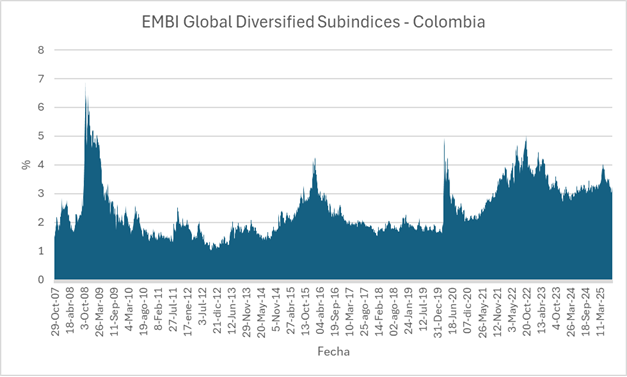
\includegraphics[width=0.92\textwidth,height=0.72\textheight,keepaspectratio]{graficas/embi.png}
\end{frame}

\begin{frame}{Riesgo País}
  \centering
  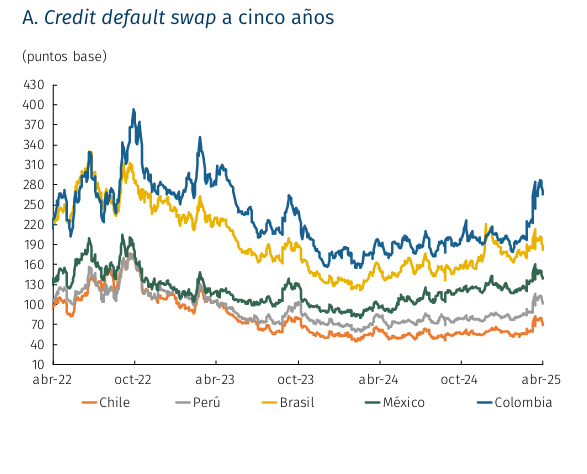
\includegraphics[width=0.90\textwidth,height=0.72\textheight,keepaspectratio]{graficas/cds.png}
\end{frame}

\begin{frame}{Riesgo País}
  \centering
  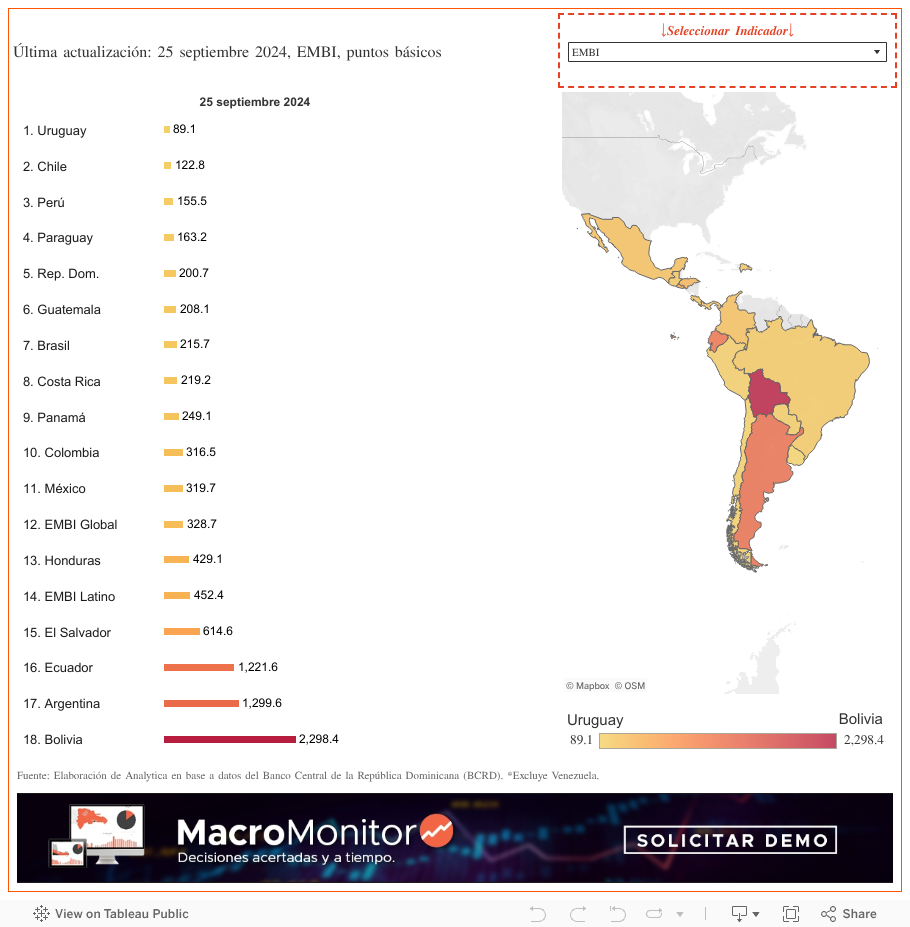
\includegraphics[width=0.90\textwidth,height=0.72\textheight,keepaspectratio]{graficas/1_rss.png}
\end{frame}
\begin{frame}{El gasto inflexible disminuyó, pero siguió cerca de 20\% del PIB}
\centering
\small
\begin{tabular}{lrrr}
\toprule
\textbf{Categoría (\% del PIB)} & \textbf{2024} & \textbf{2025} & \textbf{Cambio} \\
\midrule
Intereses                         & 4,3 & 2,8 & -1,5 \\
Gasto de personal mínimo          & 1,9 & 2,0 &  0,1 \\
Adquisición mínima de bienes y servicios & 0,4 & 0,5 & 0,1 \\
Transferencias obligatorias       & 13,3 & 13,3 & 0,0 \\
Inversión inflexible              & 0,7 & 1,1 &  0,4 \\
\midrule
\textbf{Gasto inflexible}         & \textbf{20,6} & \textbf{19,7} & \textbf{-0,9} \\
Funcionamiento discrecional       & 1,2 & 1,5 & 0,3 \\
Inversión discrecional            & 1,3 & 1,5 & 0,2 \\
\textbf{Gasto discrecional}       & \textbf{2,5} & \textbf{3,0} & \textbf{0,5} \\
\midrule
\textbf{Gasto total}              & \textbf{23,1} & \textbf{22,7} & \textbf{-0,4} \\
\bottomrule
\end{tabular}
\note{[Sources] MFMP 2026, capítulo 1, gráfico 1.7. Cálculos propios de agregación.}
\end{frame}
\begin{frame}{La deuda neta se mantendría cerca de 59\% del PIB}
\centering
\begin{tikzpicture}
\begin{axis}[
  width=0.90\textwidth,height=0.50\textwidth,
  ylabel={Deuda neta (\% del PIB)},xmin=2019,xmax=2036,ymin=45,ymax=73,
  xtick={2019,2021,...,2035},xticklabel style={rotate=90,anchor=east,/pgf/number format/.cd,1000 sep={},fixed,precision=0},scaled x ticks=false,
  ytick={45,50,...,70},grid=major,
  legend style={at={(0.5,1.02)},anchor=south,legend columns=2,font=\scriptsize}
]
\addplot[color=blue,very thick,mark=*] coordinates {
 (2019,48.4) (2020,60.7) (2021,60.0) (2022,57.6) (2023,53.3) (2024,59.0)
 (2025,58.6) (2026,58.9) (2027,58.9) (2028,59.3) (2029,59.6) (2030,59.4)
 (2031,59.1) (2032,58.8) (2033,58.5) (2034,58.3) (2035,58.0) (2036,57.6)
};
\addlegendentry{MFMP 2026}
\addplot[color=gray,dashed,thick] coordinates {
 (2019,48.4) (2020,60.7) (2021,60.0) (2022,57.6) (2023,53.4) (2024,59.0)
 (2025,61.3) (2026,63.0) (2027,63.8) (2028,63.4) (2029,63.2) (2030,62.9)
 (2031,62.3) (2032,62.0) (2033,61.7) (2034,61.6) (2035,61.4) (2036,61.3)
};
\addlegendentry{MFMP 2025}
\addplot[color=red!70!black,dotted,thick] coordinates {(2019,71) (2036,71)};
\addplot[color=green!50!black,dotted,thick] coordinates {(2019,55) (2036,55)};
\end{axis}
\end{tikzpicture}

\scriptsize Fuente: MFMP 2026, capítulo 3, gráfico 3.10. La línea gris muestra la senda publicada en el MFMP 2025.
\end{frame}
\begin{frame}{El MFMP proyecta superávit primario desde 2028}
\centering
\begin{tikzpicture}
\begin{axis}[
  width=0.90\textwidth,height=0.50\textwidth,
  ylabel={Balance primario (\% del PIB)},xmin=2019,xmax=2036,ymin=-5.5,ymax=2,
  xtick={2019,2021,...,2035},xticklabel style={rotate=90,anchor=east,/pgf/number format/.cd,1000 sep={},fixed,precision=0},scaled x ticks=false,
  ytick={-5,-4,...,2},grid=both,
  legend style={at={(0.5,1.02)},anchor=south,font=\scriptsize}
]
\addplot[color=black!35,thin,forget plot] coordinates {(2019,0) (2036,0)};
\addplot[color=blue,very thick,mark=*] coordinates {
 (2019,0.4) (2020,-4.9) (2021,-3.7) (2022,-1.0) (2023,-0.3) (2024,-2.4)
 (2025,-3.5) (2026,-2.1) (2027,-0.5) (2028,0.5) (2029,0.7) (2030,1.0)
 (2031,1.2) (2032,1.2) (2033,1.2) (2034,1.1) (2035,1.2) (2036,1.2)
};
\addlegendentry{MFMP 2026}
\end{axis}
\end{tikzpicture}

\scriptsize Fuente: MFMP 2026, capítulo 3, tabla 3.1; serie histórica 2019--2024: MHCP, como en la versión fuente.
\end{frame}
\begin{frame}
  \frametitle{Tenedores de deuda pública interna — diciembre de 2019}
  \centering
  \begin{tabular}{lr}
    \toprule
    Tenedor & Participación (\%) \\
    \midrule
    Fondos de pensiones y cesantías & 31 \\
    Fondos de capital extranjero & 24 \\
    Bancos comerciales & 15 \\
    Entidades, fiducias e instituciones públicas & 15 \\
    Compañías de seguros & 5 \\
    Otros & 10 \\
    \bottomrule
  \end{tabular}

  \vfill
  \footnotesize\textit{Fuente: cálculos con base en la Dirección de Crédito Público del Ministerio de Hacienda.}
\end{frame}

\begin{frame}
  \frametitle{Tenedores de deuda pública interna — diciembre de 2024}
  \centering
  \begin{tabular}{lr}
    \toprule
    Tenedor & Participación (\%) \\
    \midrule
    Fondos de pensiones y cesantías & 32 \\
    Fondos de capital extranjero & 18 \\
    Bancos comerciales & 16 \\
    Entidades, fiducias e instituciones públicas & 12 \\
    Compañías de seguros & 12 \\
    Otros & 10 \\
    \bottomrule
  \end{tabular}

  \vfill
  \footnotesize\textit{Fuente: cálculos con base en la Dirección de Crédito Público del Ministerio de Hacienda. El MFMP 2026 no incluye la composición de tenedores con corte de 2025.}
\end{frame}
\input{slides/PuntosConsolidacion.tex}
\input{slides/VFforecast.tex}

\section{Riesgos fiscales}
\input{slides/Nomina.tex}
\input{slides/pension_f.tex}
\input{slides/upc.tex}
\input{slides/ESGP.tex}
\input{slides/aquiles.tex}
\input{slides/Riesgos.tex}

\section{Reformas}
\begin{frame}{Reformas Institucionales}
\begin{itemize}
    \item La activación de la cláusula de escape en 2025 revela los límites del marco fiscal vigente.
    \item El problema estructural es la obligación de incluir todas las obligaciones legales de gasto sin contar con ingresos suficientes.
    \item La sobreestimación de ingresos se ha convertido en una práctica recurrente para cuadrar el presupuesto.
\end{itemize}
\end{frame}

\begin{frame}{Reformas Institucionales}
\begin{itemize}
    \item Fortalecer la Oficina de Asistencia Técnica Presupuestal para aumentar la capacidad técnica del Congreso y complementar al CARF.
    \item Dar carácter independiente y vinculante a la validación de las proyecciones de ingresos y de las obligaciones legales de gasto.
    \item Si la regla fiscal impide presupuestar todas las obligaciones legales de gasto, activar un mecanismo que obligue a definir ingresos o recortes compensatorios.
    \item Modificar el artículo 348 de la Constitución para que, si el Congreso no aprueba el PGN, se reconduzca el presupuesto anterior.
\end{itemize}
\end{frame}

\begin{frame}{Reformas Institucionales}
\begin{itemize}
    \item Unificar los presupuestos de funcionamiento e inversión en el Ministerio de Hacienda.
    \item Medir la ejecución presupuestal sin contar como ejecución las transferencias a fiducias y patrimonios autónomos.
    \item Reformar las pérdidas de apropiación para permitir el traslado parcial de saldos no comprometidos.
    \item Dejar la clasificación de transacciones de única vez a cargo exclusivo del CARF.
    \item Garantizar acceso público y auditable al detalle del cierre fiscal.
\end{itemize}
\end{frame}
\input{slides/solINV.tex}
\begin{frame}{Subsidio a los combustibles}
\begin{itemize}
  \item La transferencia al FEPC bajó de \textbf{1,7\% del PIB en 2023} a \textbf{1,2\% en 2024} y \textbf{0,4\% en 2025}.
  \item La reducción de 0,8 puntos del PIB en 2025 compensó parcialmente el aumento de otras transferencias obligatorias.
  \item Eliminar el déficit remanente exige cerrar la brecha del diésel, con costos políticos, sociales y de orden público.
  \item La consolidación futura depende de evitar una nueva acumulación de obligaciones en el fondo.
\end{itemize}
\note{[Sources] MFMP 2026, capítulo 1, gráfico 1.7.}
\end{frame}
\begin{frame}{Salud}
\begin{itemize}
    \item Excluir tratamientos de bajo impacto o alto costo.
    \item Sistematizar y centralizar la información de pacientes y tratamientos para mejorar la gestión.
\end{itemize}
\end{frame}

\begin{frame}{Salud}
\begin{itemize}
    \item Transitar hacia competencia en primas entre EPS para incentivar la eficiencia.
    \item Aumentar la financiación territorial en el marco de la Ley de Competencias.
    \item Redirigir contribuciones de las cajas de compensación al sistema de salud.
\end{itemize}
\end{frame}

\begin{frame}{Salud}
\begin{itemize}
    \item Aumentar la cotización a salud de los pensionados al 16\%.
    \item Financiar parte del sistema con impuestos generales, incluida una ampliación de la base del IVA con compensación a hogares vulnerables.
    \item Reconocer que la presión fiscal seguirá aumentando por el envejecimiento y la incorporación de nuevas tecnologías.
\end{itemize}
\end{frame}
\begin{frame}{Pensiones}
\begin{itemize}
    \item El gasto pensional incluye a Colpensiones y a los regímenes especiales de las Fuerzas Militares, los docentes y otros empleados públicos.
    \item Entre 2024 y 2035, el gasto en pensiones podría aumentar cerca de 1 punto del PIB.
    \item La cobertura sigue siendo baja: solo uno de cada cuatro adultos mayores recibe pensión.
\end{itemize}
\end{frame}

\begin{frame}{Pensiones}
\begin{enumerate}
    \item Ajustes paramétricos:
    \begin{itemize}
        \item edad de pensión;
        \item tasa de reemplazo;
        \item umbral de cotización.
    \end{itemize}
    \item Eliminar la exención de impuestos a las pensiones.
    \item Aumentar la cotización en salud de los pensionados.
    \item Incrementar los aportes de los pensionados al Fondo de Solidaridad Pensional.
\end{enumerate}
\end{frame}

\begin{frame}{Pensiones}
\begin{itemize}
    \item La Ley 2381 de 2024 dirige más cotizaciones al componente público y crea un fondo de ahorro administrado por el Banco de la República.
    \item El uso de los recursos del fondo ante presiones fiscales adelantaría su agotamiento.
    \item Los ajustes al umbral de ingresos, la tasa de reemplazo y la edad de jubilación deben evaluarse por cohortes.
    \item Una reforma temprana reduciría el pasivo implícito y enviaría una señal de compromiso fiscal.
\end{itemize}
\end{frame}
\begin{frame}{Las competencias transferibles equivalen a cerca de 5,3\% del PIB}
\centering
\small
\begin{tabular}{lr}
\toprule
\textbf{Competencia, estimación 2025} & \textbf{\% del PIB} \\
\midrule
Inversión                              & 2,6 \\
Aseguramiento en salud                 & 2,0 \\
SENA e ICBF                            & 0,3 \\
Universidades públicas                 & 0,4 \\
\midrule
\textbf{Total}                         & \textbf{5,3} \\
\bottomrule
\end{tabular}
\vspace{0.25cm}
\scriptsize La transferencia de recursos solo es fiscalmente neutral si viene acompañada de competencias por un valor equivalente.
\note{[Sources] MFMP 2026, capítulo 1, gráfico 1.7, para inversión y salud. SENA, ICBF y universidades: clasificación MHCP/CARF conservada de la versión fuente.}
\end{frame}
\input{slides/solSGP.tex}
\input{slides/MasSGP.tex}

\section{Viabilidad política del ajuste}
\input{slides/ComentariosFinales.tex}

\section{Comentarios finales}
\input{slides/conclusiones.tex}

\begin{frame}{}
  \begin{columns}[c]
    \column{0.45\textwidth}
    \centering
    
\includegraphics[width=\textwidth,height=0.62\textheight,keepaspectratio]{graficas/Cover.jpg}

    \column{0.55\textwidth}
    \centering
    {\Large\textbf{Muchas gracias}}

    \vspace{0.5cm}
    \small
    Oliver Pardo\\
    Centro Javeriano de Competitividad\\
    Pontificia Universidad Javeriana

    \vspace{0.5cm}
    \footnotesize
    pardoo@javeriana.edu.co\\
    X: @opardor
  \end{columns}
\end{frame}

\end{document}